%%%%%%%%%%%%%%%%%%%%%%%%%%%%%%%%%%%%%%%%%
% The Legrand Orange Book
% LaTeX Template
% Version 2.0 (9/2/15)
%
% This template has been downloaded from:
% http://www.LaTeXTemplates.com
%
% Mathias Legrand (legrand.mathias@gmail.com) with modifications by:
% Vel (vel@latextemplates.com)
%
% License:
% CC BY-NC-SA 3.0 (http://creativecommons.org/licenses/by-nc-sa/3.0/)
%
% Compiling this template:
% This template uses biber for its bibliography and makeindex for its index.
% When you first open the template, compile it from the command line with the 
% commands below to make sure your LaTeX distribution is configured correctly:
%
% 1) pdflatex main
% 2) makeindex main.idx -s StyleInd.ist
% 3) biber main
% 4) pdflatex main x 2
%
% After this, when you wish to update the bibliography/index use the appropriate
% command above and make sure to compile with pdflatex several times 
% afterwards to propagate your changes to the document.
%
% This template also uses a number of packages which may need to be
% updated to the newest versions for the template to compile. It is strongly
% recommended you update your LaTeX distribution if you have any
% compilation errors.
%
% Important note:
% Chapter heading images should have a 2:1 width:height ratio,
% e.g. 920px width and 460px height.
%
%%%%%%%%%%%%%%%%%%%%%%%%%%%%%%%%%%%%%%%%%

%----------------------------------------------------------------------------------------
%	PACKAGES AND OTHER DOCUMENT CONFIGURATIONS
%----------------------------------------------------------------------------------------

\documentclass[11pt,fleqn]{book} % Default font size and left-justified equations

\usepackage{mathrsfs}
\usepackage{amsbsy}
\usepackage{multicol}
\usepackage{graphicx}
\usepackage{bm}

\newcommand{\indep}{\rotatebox[origin=c]{90}{$\models$}}
%----------------------------------------------------------------------------------------

%fdlkjadlkjdfsal;kjafds;lkjafsd;lkjfsad

%%%%%%%%%%%%%%%%%%%%%%%%%%%%%%%%%%%%%%%%%
% The Legrand Orange Book
% Structural Definitions File
% Version 2.0 (9/2/15)
%
% Original author:
% Mathias Legrand (legrand.mathias@gmail.com) with modifications by:
% Vel (vel@latextemplates.com)
% 
% This file has been downloaded from:
% http://www.LaTeXTemplates.com
%
% License:
% CC BY-NC-SA 3.0 (http://creativecommons.org/licenses/by-nc-sa/3.0/)
%
%%%%%%%%%%%%%%%%%%%%%%%%%%%%%%%%%%%%%%%%%

%----------------------------------------------------------------------------------------
%	VARIOUS REQUIRED PACKAGES AND CONFIGURATIONS
%----------------------------------------------------------------------------------------

\usepackage[top=3cm,bottom=3cm,left=3cm,right=3cm,headsep=10pt,a4paper]{geometry} % Page margins

\usepackage{graphicx} % Required for including pictures
\graphicspath{{Pictures/}} % Specifies the directory where pictures are stored

\usepackage{lipsum} % Inserts dummy text

\usepackage{tikz} % Required for drawing custom shapes

\usepackage[english]{babel} % English language/hyphenation

\usepackage{enumitem} % Customize lists
\setlist{nolistsep} % Reduce spacing between bullet points and numbered lists

\usepackage{booktabs} % Required for nicer horizontal rules in tables

\usepackage{xcolor} % Required for specifying colors by name
\definecolor{ocre}{RGB}{243,102,25} % Define the orange color used for highlighting throughout the book

%----------------------------------------------------------------------------------------
%	FONTS
%----------------------------------------------------------------------------------------

\usepackage{avant} % Use the Avantgarde font for headings
%\usepackage{times} % Use the Times font for headings
\usepackage{mathptmx} % Use the Adobe Times Roman as the default text font together with math symbols from the Sym­bol, Chancery and Com­puter Modern fonts

\usepackage{microtype} % Slightly tweak font spacing for aesthetics
\usepackage[utf8]{inputenc} % Required for including letters with accents
\usepackage[T1]{fontenc} % Use 8-bit encoding that has 256 glyphs

%----------------------------------------------------------------------------------------
%	BIBLIOGRAPHY AND INDEX
%----------------------------------------------------------------------------------------

\usepackage[style=alphabetic,citestyle=numeric,sorting=nyt,sortcites=true,autopunct=true,babel=hyphen,hyperref=true,abbreviate=false,backref=true,backend=biber]{biblatex}
\addbibresource{bibliography.bib} % BibTeX bibliography file
\defbibheading{bibempty}{}

\usepackage{calc} % For simpler calculation - used for spacing the index letter headings correctly
\usepackage{makeidx} % Required to make an index
\makeindex % Tells LaTeX to create the files required for indexing

%----------------------------------------------------------------------------------------
%	MAIN TABLE OF CONTENTS
%----------------------------------------------------------------------------------------

\usepackage{titletoc} % Required for manipulating the table of contents

\contentsmargin{0cm} % Removes the default margin

% Part text styling
\titlecontents{part}[0cm]
{\addvspace{20pt}\centering\large\bfseries}
{}
{}
{}

% Chapter text styling
\titlecontents{chapter}[1.25cm] % Indentation
{\addvspace{12pt}\large\sffamily\bfseries} % Spacing and font options for chapters
{\color{ocre!60}\contentslabel[\Large\thecontentslabel]{1.25cm}\color{ocre}} % Chapter number
{\color{ocre}}  
{\color{ocre!60}\normalsize\;\titlerule*[.5pc]{.}\;\thecontentspage} % Page number

% Section text styling
\titlecontents{section}[1.25cm] % Indentation
{\addvspace{3pt}\sffamily\bfseries} % Spacing and font options for sections
{\contentslabel[\thecontentslabel]{1.25cm}} % Section number
{}
{\hfill\color{black}\thecontentspage} % Page number
[]

% Subsection text styling
\titlecontents{subsection}[1.25cm] % Indentation
{\addvspace{1pt}\sffamily\small} % Spacing and font options for subsections
{\contentslabel[\thecontentslabel]{1.25cm}} % Subsection number
{}
{\ \titlerule*[.5pc]{.}\;\thecontentspage} % Page number
[]

% List of figures
\titlecontents{figure}[0em]
{\addvspace{-5pt}\sffamily}
{\thecontentslabel\hspace*{1em}}
{}
{\ \titlerule*[.5pc]{.}\;\thecontentspage}
[]

% List of tables
\titlecontents{table}[0em]
{\addvspace{-5pt}\sffamily}
{\thecontentslabel\hspace*{1em}}
{}
{\ \titlerule*[.5pc]{.}\;\thecontentspage}
[]

%----------------------------------------------------------------------------------------
%	MINI TABLE OF CONTENTS IN PART HEADS
%----------------------------------------------------------------------------------------

% Chapter text styling
\titlecontents{lchapter}[0em] % Indenting
{\addvspace{15pt}\large\sffamily\bfseries} % Spacing and font options for chapters
{\color{ocre}\contentslabel[\Large\thecontentslabel]{1.25cm}\color{ocre}} % Chapter number
{}  
{\color{ocre}\normalsize\sffamily\bfseries\;\titlerule*[.5pc]{.}\;\thecontentspage} % Page number

% Section text styling
\titlecontents{lsection}[0em] % Indenting
{\sffamily\small} % Spacing and font options for sections
{\contentslabel[\thecontentslabel]{1.25cm}} % Section number
{}
{}

% Subsection text styling
\titlecontents{lsubsection}[.5em] % Indentation
{\normalfont\footnotesize\sffamily} % Font settings
{}
{}
{}

%----------------------------------------------------------------------------------------
%	PAGE HEADERS
%----------------------------------------------------------------------------------------

\usepackage{fancyhdr} % Required for header and footer configuration

\pagestyle{fancy}
\renewcommand{\chaptermark}[1]{\markboth{\sffamily\normalsize\bfseries\chaptername\ \thechapter.\ #1}{}} % Chapter text font settings
\renewcommand{\sectionmark}[1]{\markright{\sffamily\normalsize\thesection\hspace{5pt}#1}{}} % Section text font settings
\fancyhf{} \fancyhead[LE,RO]{\sffamily\normalsize\thepage} % Font setting for the page number in the header
\fancyhead[LO]{\rightmark} % Print the nearest section name on the left side of odd pages
\fancyhead[RE]{\leftmark} % Print the current chapter name on the right side of even pages
\renewcommand{\headrulewidth}{0.5pt} % Width of the rule under the header
\addtolength{\headheight}{2.5pt} % Increase the spacing around the header slightly
\renewcommand{\footrulewidth}{0pt} % Removes the rule in the footer
\fancypagestyle{plain}{\fancyhead{}\renewcommand{\headrulewidth}{0pt}} % Style for when a plain pagestyle is specified

% Removes the header from odd empty pages at the end of chapters
\makeatletter
\renewcommand{\cleardoublepage}{
\clearpage\ifodd\c@page\else
\hbox{}
\vspace*{\fill}
\thispagestyle{empty}
\newpage
\fi}

%----------------------------------------------------------------------------------------
%	THEOREM STYLES
%----------------------------------------------------------------------------------------

\usepackage{amsmath,amsfonts,amssymb,amsthm} % For math equations, theorems, symbols, etc

\newcommand{\intoo}[2]{\mathopen{]}#1\,;#2\mathclose{[}}
\newcommand{\ud}{\mathop{\mathrm{{}d}}\mathopen{}}
\newcommand{\intff}[2]{\mathopen{[}#1\,;#2\mathclose{]}}
\newtheorem{notation}{Notation}[chapter]

% Boxed/framed environments
\newtheoremstyle{ocrenumbox}% % Theorem style name
{0pt}% Space above
{0pt}% Space below
{\normalfont}% % Body font
{}% Indent amount
{\small\bf\sffamily\color{ocre}}% % Theorem head font
{\;}% Punctuation after theorem head
{0.25em}% Space after theorem head
{\small\sffamily\color{ocre}\thmname{#1}\nobreakspace\thmnumber{\@ifnotempty{#1}{}\@upn{#2}}% Theorem text (e.g. Theorem 2.1)
\thmnote{\nobreakspace\the\thm@notefont\sffamily\bfseries\color{black}---\nobreakspace#3.}} % Optional theorem note
\renewcommand{\qedsymbol}{$\blacksquare$}% Optional qed square

\newtheoremstyle{blacknumex}% Theorem style name
{5pt}% Space above
{5pt}% Space below
{\normalfont}% Body font
{} % Indent amount
{\small\bf\sffamily}% Theorem head font
{\;}% Punctuation after theorem head
{0.25em}% Space after theorem head
{\small\sffamily{\tiny\ensuremath{\blacksquare}}\nobreakspace\thmname{#1}\nobreakspace\thmnumber{\@ifnotempty{#1}{}\@upn{#2}}% Theorem text (e.g. Theorem 2.1)
\thmnote{\nobreakspace\the\thm@notefont\sffamily\bfseries---\nobreakspace#3.}}% Optional theorem note

\newtheoremstyle{blacknumbox} % Theorem style name
{0pt}% Space above
{0pt}% Space below
{\normalfont}% Body font
{}% Indent amount
{\small\bf\sffamily}% Theorem head font
{\;}% Punctuation after theorem head
{0.25em}% Space after theorem head
{\small\sffamily\thmname{#1}\nobreakspace\thmnumber{\@ifnotempty{#1}{}\@upn{#2}}% Theorem text (e.g. Theorem 2.1)
\thmnote{\nobreakspace\the\thm@notefont\sffamily\bfseries---\nobreakspace#3.}}% Optional theorem note

% Non-boxed/non-framed environments
\newtheoremstyle{ocrenum}% % Theorem style name
{5pt}% Space above
{5pt}% Space below
{\normalfont}% % Body font
{}% Indent amount
{\small\bf\sffamily\color{ocre}}% % Theorem head font
{\;}% Punctuation after theorem head
{0.25em}% Space after theorem head
{\small\sffamily\color{ocre}\thmname{#1}\nobreakspace\thmnumber{\@ifnotempty{#1}{}\@upn{#2}}% Theorem text (e.g. Theorem 2.1)
\thmnote{\nobreakspace\the\thm@notefont\sffamily\bfseries\color{black}---\nobreakspace#3.}} % Optional theorem note
\renewcommand{\qedsymbol}{$\blacksquare$}% Optional qed square
\makeatother

% Defines the theorem text style for each type of theorem to one of the three styles above
\newcounter{dummy} 
\numberwithin{dummy}{section}
\theoremstyle{ocrenumbox}
\newtheorem{theoremeT}[dummy]{Theorem}
\newtheorem{problem}{Problem}[chapter]
\newtheorem{exerciseT}{Exercise}[chapter]
\theoremstyle{blacknumex}
\newtheorem{exampleT}{Example}[chapter]
\theoremstyle{blacknumbox}
\newtheorem{vocabulary}{Vocabulary}[chapter]
\newtheorem{definitionT}{Definition}[section]
\newtheorem{corollaryT}[dummy]{Corollary}
\theoremstyle{ocrenum}
\newtheorem{proposition}[dummy]{Proposition}

%----------------------------------------------------------------------------------------
%	DEFINITION OF COLORED BOXES
%----------------------------------------------------------------------------------------

\RequirePackage[framemethod=default]{mdframed} % Required for creating the theorem, definition, exercise and corollary boxes

% Theorem box
\newmdenv[skipabove=7pt,
skipbelow=7pt,
backgroundcolor=black!5,
linecolor=ocre,
innerleftmargin=5pt,
innerrightmargin=5pt,
innertopmargin=5pt,
leftmargin=0cm,
rightmargin=0cm,
innerbottommargin=5pt]{tBox}

% Exercise box	  
\newmdenv[skipabove=7pt,
skipbelow=7pt,
rightline=false,
leftline=true,
topline=false,
bottomline=false,
backgroundcolor=ocre!10,
linecolor=ocre,
innerleftmargin=5pt,
innerrightmargin=5pt,
innertopmargin=5pt,
innerbottommargin=5pt,
leftmargin=0cm,
rightmargin=0cm,
linewidth=4pt]{eBox}	

% Definition box
\newmdenv[skipabove=7pt,
skipbelow=7pt,
rightline=false,
leftline=true,
topline=false,
bottomline=false,
linecolor=ocre,
innerleftmargin=5pt,
innerrightmargin=5pt,
innertopmargin=0pt,
leftmargin=0cm,
rightmargin=0cm,
linewidth=4pt,
innerbottommargin=0pt]{dBox}	

% Corollary box
\newmdenv[skipabove=7pt,
skipbelow=7pt,
rightline=false,
leftline=true,
topline=false,
bottomline=false,
linecolor=gray,
backgroundcolor=black!5,
innerleftmargin=5pt,
innerrightmargin=5pt,
innertopmargin=5pt,
leftmargin=0cm,
rightmargin=0cm,
linewidth=4pt,
innerbottommargin=5pt]{cBox}

% Creates an environment for each type of theorem and assigns it a theorem text style from the "Theorem Styles" section above and a colored box from above
\newenvironment{theorem}{\begin{tBox}\begin{theoremeT}}{\end{theoremeT}\end{tBox}}
\newenvironment{exercise}{\begin{eBox}\begin{exerciseT}}{\hfill{\color{ocre}\tiny\ensuremath{\blacksquare}}\end{exerciseT}\end{eBox}}				  
\newenvironment{definition}{\begin{dBox}\begin{definitionT}}{\end{definitionT}\end{dBox}}	
\newenvironment{example}{\begin{exampleT}}{\hfill{\tiny\ensuremath{\blacksquare}}\end{exampleT}}		
\newenvironment{corollary}{\begin{cBox}\begin{corollaryT}}{\end{corollaryT}\end{cBox}}	

%----------------------------------------------------------------------------------------
%	REMARK ENVIRONMENT
%----------------------------------------------------------------------------------------

\newenvironment{remark}{\par\vspace{10pt}\small % Vertical white space above the remark and smaller font size
\begin{list}{}{
\leftmargin=35pt % Indentation on the left
\rightmargin=25pt}\item\ignorespaces % Indentation on the right
\makebox[-2.5pt]{\begin{tikzpicture}[overlay]
\node[draw=ocre!60,line width=1pt,circle,fill=ocre!25,font=\sffamily\bfseries,inner sep=2pt,outer sep=0pt] at (-15pt,0pt){\textcolor{ocre}{R}};\end{tikzpicture}} % Orange R in a circle
\advance\baselineskip -1pt}{\end{list}\vskip5pt} % Tighter line spacing and white space after remark

%----------------------------------------------------------------------------------------
%	SECTION NUMBERING IN THE MARGIN
%----------------------------------------------------------------------------------------

\makeatletter
\renewcommand{\@seccntformat}[1]{\llap{\textcolor{ocre}{\csname the#1\endcsname}\hspace{1em}}}                    
\renewcommand{\section}{\@startsection{section}{1}{\z@}
{-4ex \@plus -1ex \@minus -.4ex}
{1ex \@plus.2ex }
{\normalfont\large\sffamily\bfseries}}
\renewcommand{\subsection}{\@startsection {subsection}{2}{\z@}
{-3ex \@plus -0.1ex \@minus -.4ex}
{0.5ex \@plus.2ex }
{\normalfont\sffamily\bfseries}}
\renewcommand{\subsubsection}{\@startsection {subsubsection}{3}{\z@}
{-2ex \@plus -0.1ex \@minus -.2ex}
{.2ex \@plus.2ex }
{\normalfont\small\sffamily\bfseries}}                        
\renewcommand\paragraph{\@startsection{paragraph}{4}{\z@}
{-2ex \@plus-.2ex \@minus .2ex}
{.1ex}
{\normalfont\small\sffamily\bfseries}}

%----------------------------------------------------------------------------------------
%	PART HEADINGS
%----------------------------------------------------------------------------------------

% numbered part in the table of contents
\newcommand{\@mypartnumtocformat}[2]{%
\setlength\fboxsep{0pt}%
\noindent\colorbox{ocre!20}{\strut\parbox[c][.7cm]{\ecart}{\color{ocre!70}\Large\sffamily\bfseries\centering#1}}\hskip\esp\colorbox{ocre!40}{\strut\parbox[c][.7cm]{\linewidth-\ecart-\esp}{\Large\sffamily\centering#2}}}%
%%%%%%%%%%%%%%%%%%%%%%%%%%%%%%%%%%
% unnumbered part in the table of contents
\newcommand{\@myparttocformat}[1]{%
\setlength\fboxsep{0pt}%
\noindent\colorbox{ocre!40}{\strut\parbox[c][.7cm]{\linewidth}{\Large\sffamily\centering#1}}}%
%%%%%%%%%%%%%%%%%%%%%%%%%%%%%%%%%%
\newlength\esp
\setlength\esp{4pt}
\newlength\ecart
\setlength\ecart{1.2cm-\esp}
\newcommand{\thepartimage}{}%
\newcommand{\partimage}[1]{\renewcommand{\thepartimage}{#1}}%
\def\@part[#1]#2{%
\ifnum \c@secnumdepth >-2\relax%
\refstepcounter{part}%
\addcontentsline{toc}{part}{\texorpdfstring{\protect\@mypartnumtocformat{\thepart}{#1}}{\partname~\thepart\ ---\ #1}}
\else%
\addcontentsline{toc}{part}{\texorpdfstring{\protect\@myparttocformat{#1}}{#1}}%
\fi%
\startcontents%
\markboth{}{}%
{\thispagestyle{empty}%
\begin{tikzpicture}[remember picture,overlay]%
\node at (current page.north west){\begin{tikzpicture}[remember picture,overlay]%	
\fill[ocre!20](0cm,0cm) rectangle (\paperwidth,-\paperheight);
\node[anchor=north] at (4cm,-3.25cm){\color{ocre!40}\fontsize{220}{100}\sffamily\bfseries\@Roman\c@part}; 
\node[anchor=south east] at (\paperwidth-1cm,-\paperheight+1cm){\parbox[t][][t]{8.5cm}{
\printcontents{l}{0}{\setcounter{tocdepth}{1}}%
}};
\node[anchor=north east] at (\paperwidth-1.5cm,-3.25cm){\parbox[t][][t]{15cm}{\strut\raggedleft\color{white}\fontsize{30}{30}\sffamily\bfseries#2}};
\end{tikzpicture}};
\end{tikzpicture}}%
\@endpart}
\def\@spart#1{%
\startcontents%
\phantomsection
{\thispagestyle{empty}%
\begin{tikzpicture}[remember picture,overlay]%
\node at (current page.north west){\begin{tikzpicture}[remember picture,overlay]%	
\fill[ocre!20](0cm,0cm) rectangle (\paperwidth,-\paperheight);
\node[anchor=north east] at (\paperwidth-1.5cm,-3.25cm){\parbox[t][][t]{15cm}{\strut\raggedleft\color{white}\fontsize{30}{30}\sffamily\bfseries#1}};
\end{tikzpicture}};
\end{tikzpicture}}
\addcontentsline{toc}{part}{\texorpdfstring{%
\setlength\fboxsep{0pt}%
\noindent\protect\colorbox{ocre!40}{\strut\protect\parbox[c][.7cm]{\linewidth}{\Large\sffamily\protect\centering #1\quad\mbox{}}}}{#1}}%
\@endpart}
\def\@endpart{\vfil\newpage
\if@twoside
\if@openright
\null
\thispagestyle{empty}%
\newpage
\fi
\fi
\if@tempswa
\twocolumn
\fi}

%----------------------------------------------------------------------------------------
%	CHAPTER HEADINGS
%----------------------------------------------------------------------------------------

\newcommand{\thechapterimage}{}%
\newcommand{\chapterimage}[1]{\renewcommand{\thechapterimage}{#1}}%
\def\@makechapterhead#1{%
{\parindent \z@ \raggedright \normalfont
\ifnum \c@secnumdepth >\m@ne
\if@mainmatter
\begin{tikzpicture}[remember picture,overlay]
\node at (current page.north west)
{\begin{tikzpicture}[remember picture,overlay]
\node[anchor=north west,inner sep=0pt] at (0,0) {\includegraphics[width=\paperwidth]{\thechapterimage}};
\draw[anchor=west] (\Gm@lmargin,-9cm) node [line width=2pt,rounded corners=15pt,draw=ocre,fill=white,fill opacity=0.5,inner sep=15pt]{\strut\makebox[22cm]{}};
\draw[anchor=west] (\Gm@lmargin+.3cm,-9cm) node {\huge\sffamily\bfseries\color{black}\thechapter. #1\strut};
\end{tikzpicture}};
\end{tikzpicture}
\else
\begin{tikzpicture}[remember picture,overlay]
\node at (current page.north west)
{\begin{tikzpicture}[remember picture,overlay]
\node[anchor=north west,inner sep=0pt] at (0,0) {\includegraphics[width=\paperwidth]{\thechapterimage}};
\draw[anchor=west] (\Gm@lmargin,-9cm) node [line width=2pt,rounded corners=15pt,draw=ocre,fill=white,fill opacity=0.5,inner sep=15pt]{\strut\makebox[22cm]{}};
\draw[anchor=west] (\Gm@lmargin+.3cm,-9cm) node {\huge\sffamily\bfseries\color{black}#1\strut};
\end{tikzpicture}};
\end{tikzpicture}
\fi\fi\par\vspace*{270\p@}}}

%-------------------------------------------

\def\@makeschapterhead#1{%
\begin{tikzpicture}[remember picture,overlay]
\node at (current page.north west)
{\begin{tikzpicture}[remember picture,overlay]
\node[anchor=north west,inner sep=0pt] at (0,0) {\includegraphics[width=\paperwidth]{\thechapterimage}};
\draw[anchor=west] (\Gm@lmargin,-9cm) node [line width=2pt,rounded corners=15pt,draw=ocre,fill=white,fill opacity=0.5,inner sep=15pt]{\strut\makebox[22cm]{}};
\draw[anchor=west] (\Gm@lmargin+.3cm,-9cm) node {\huge\sffamily\bfseries\color{black}#1\strut};
\end{tikzpicture}};
\end{tikzpicture}
\par\vspace*{270\p@}}
\makeatother

%----------------------------------------------------------------------------------------
%	HYPERLINKS IN THE DOCUMENTS
%----------------------------------------------------------------------------------------

\usepackage{hyperref}
\hypersetup{hidelinks,backref=true,pagebackref=true,hyperindex=true,colorlinks=false,breaklinks=true,urlcolor= ocre,bookmarks=true,bookmarksopen=false,pdftitle={Title},pdfauthor={Author}}
\usepackage{bookmark}
\bookmarksetup{
open,
numbered,
addtohook={%
\ifnum\bookmarkget{level}=0 % chapter
\bookmarksetup{bold}%
\fi
\ifnum\bookmarkget{level}=-1 % part
\bookmarksetup{color=ocre,bold}%
\fi
}
}
 % Insert the commands.tex file which contains the majority of the structure behind the template

\begin{document}

%----------------------------------------------------------------------------------------
%	TITLE PAGE
%----------------------------------------------------------------------------------------

\begingroup
\thispagestyle{empty}
\begin{tikzpicture}[remember picture,overlay]
\coordinate [below=12cm] (midpoint) at (current page.north);
\node at (current page.north west)
{\begin{tikzpicture}[remember picture,overlay]
\node[anchor=north west,inner sep=0pt] at (0,0) {
\includegraphics[width=\paperwidth]{background}}; % Background image
\draw[anchor=north] (midpoint) node [fill=ocre!30!white,fill opacity=0.6,text opacity=1,inner sep=1cm]{\Huge\centering\bfseries\sffamily\parbox[c][][t]{\paperwidth}{\centering Linear Models\\[15pt] % Book title
{\Large STAT 551}\\[20pt] % Subtitle
{\huge Course Notes by Meridith Bartley}}}; % Author name
\end{tikzpicture}};
\end{tikzpicture}
\vfill
\endgroup

%----------------------------------------------------------------------------------------
%	COPYRIGHT PAGE
%----------------------------------------------------------------------------------------

\newpage
~\vfill
\thispagestyle{empty}

\noindent Copyright \copyright\ 2013 John Smith\\ % Copyright notice

\noindent \textsc{Published by Publisher}\\ % Publisher

\noindent \textsc{book-website.com}\\ % URL

\noindent Licensed under the Creative Commons Attribution-NonCommercial 3.0 Unported License (the ``License''). You may not use this file except in compliance with the License. You may obtain a copy of the License at \url{http://creativecommons.org/licenses/by-nc/3.0}. Unless required by applicable law or agreed to in writing, software distributed under the License is distributed on an \textsc{``as is'' basis, without warranties or conditions of any kind}, either express or implied. See the License for the specific language governing permissions and limitations under the License.\\ % License information

\noindent \textit{First printing, March 2013} % Printing/edition date

%----------------------------------------------------------------------------------------
%	TABLE OF CONTENTS
%----------------------------------------------------------------------------------------

\chapterimage{chapter_head_1.pdf} % Table of contents heading image

\pagestyle{empty} % No headers

\tableofcontents % Print the table of contents itself

\cleardoublepage % Forces the first chapter to start on an odd page so it's on the right

\pagestyle{fancy} % Print headers again

%----------------------------------------------------------------------------------------
%	PART
%----------------------------------------------------------------------------------------

\part{Part One}

%----------------------------------------------------------------------------------------
%	CHAPTER 1
%----------------------------------------------------------------------------------------

\chapterimage{chapter_head_2.pdf} % Chapter heading image

\chapter{Linear Regression}


\begin{itemize}
	\item projection
	\item orthongonal decomposition
	\item Gaussian Linear Regression
	\item prediction (generally of $\hat{y}$)
	\item different types of errors
	\item  influence 
	\item lack of fit
	\item $R^2$
	\item Multicollinearity

\end{itemize}

\section{Projection in Euclidean Space}\index{Projection}

\textbf{Monday August 22}

\begin{definition}[Euclidian Space]
	One way to think of the Euclidean plane is as a set of points satisfying certain relationships, expressible in terms of distance and angle. \textbf{Euclidean space} is an abstraction detached from actual physical locations, specific reference frames, measurement instruments, and so on.\\
\\
	Let Euclidian Space be denoted by $\mathbb{R}^P$. \\ 

	$\mathbb{R}X \dots X\mathbb{R} = \{(x_1, \dots, x_p): x_1 \in \mathbb{R} \dots, x_p \in \mathbb{R}^P\} $
\end{definition}


\begin{definition}[Inner Product]
In linear algebra, an inner product space is a vector space with an additional structure called an inner product. This additional structure associates each pair of vectors in the space with a scalar quantity known as the inner product of the vectors. \textbf{Inner products} allow the rigorous introduction of intuitive geometrical notions such as the length of a vector or the angle between two vectors. They also provide the means of defining orthogonality between vectors (zero inner product).\\
\\
	Let $a \in \mathbb{R}^P,  b \in \mathbb{R}^P$\\
$$ a^Tb = \displaystyle\sum^{P}_{i = 1} a_i b_i$$\\
$$a^Tb =<a,b>$$
\end{definition}

 \begin{definition}[Hilbert Space]
 The mathematical concept of a Hilbert space generalizes the notion of Euclidean space. It extends the methods of vector algebra and calculus from the two-dimensional Euclidean plane and three-dimensional space to spaces with any finite or infinite number of dimensions. A Hilbert space is an abstract vector space possessing the structure of an inner product that allows length and angle to be measured. Furthermore, Hilbert spaces are complete: there are enough limits in the space to allow the techniques of calculus to be used.

 \textit{Hilbert Inner Product Space }$\{\mathbb{R}^P, <a, b>\} $ 

 	
 \end{definition}


\textbf{General Inner Product}

Let $\Sigma \in \mathbb{R}^{PxP} $ set of all $PxP$ matrices. Assume $\Sigma$  is a positive definite matrix. 

$$x^T \Sigma x <0 $$
$$\forall x \in \mathbb{R}^P$$
$$ x \neq 0$$

Then $a^T \Sigma b$ also satisfies the conditions for inner product. 

$$a^T \Sigma b = <a,b>_\Sigma$$

$$a^Tb = a^TIb = <a,b>_I$$

$\{ \mathbb{R}^P, <,>_\Sigma \}$ is a more general inner product space. \\
\\ 

\textbf{Linear Transformation}

A matrix, $A, \in \mathbb{R}^{PxP}$ can be viewed as linear transformation

$T_A: \mathbb{R}^P \rightarrow \mathbb{R}^P, x \mapsto Ax$

\begin{remark}
	Bing Li will denote $T_A$ as $A$. \\
	$\rightarrow$ means maps to for a domain.\\
	$\mapsto$ means maps to for a value.\\
	$\Rightarrow$ means implies. \\
	
\end{remark}



If $A: \mathbb{R}^P \rightarrow \mathbb{R}^P$, 

	$$ker(A) = \{x \in \mathbb{R}^P, Ax = 0 \}$$
	$$ran(A) = \{ Ax: x \in \mathbb{R}^P \}$$

\begin{definition}[Kernel]
 In linear algebra, the kernel, or sometimes the null space, is the set of all elements v of V for which L(v) = 0, where 0 denotes the zero vector in W.

 In coordinate plane, think of a function that crosses the x-axis. The kernel would be all points on x where $y=0$.
	
\end{definition}

\begin{definition}[Range]

In coordinate plane, how much of the y axis is reached with the function? Now extend this idea to more dimensions. 
	
\end{definition}

A linear transformation is \textbf{idempotent} if 

	$$A = A^2$$
	$$Ax = A(A(x)) $$
	$$\forall x \in \mathbb{R}^P$$


If A were a number it could only be 1 or 0. \\
 % get from photo
 % get arrow defintions
\\
\textbf{Wednesday August 24}

Let $T \in \mathbb{R}^{PxP}$ then there exists a unique operator $R \in \mathbb{R}^{PxP}$ such that $\forall x, y \in \mathbb{R}^P$,\\
 $$<x, Ty> = <Rx, y> $$ (general inner product, $a^T\Sigma b$). Aside: What this states is that if you give me any operator in the first you can find one in the second.\\ 
\\
$R$ is called the \textbf{adjoint operator} of T. Written as $T^*$, that is, 
 $$<x, Ty> = <T^*x, y>$$
\\
\textbf{Derived Facts}

\begin{multicols}{2}

 \begin{align*}
	<x, Ty> &= <T^*, y>\\
	&= <y, T^*x>\\
	&= <(T^*)^*y, x>\\
	&= <x, (T^*)^*y>\\
\end{align*}

\columnbreak


		(by the definition)\\
    (inner products the order doesn't matter)\\
    (Use the definition again)\\
    (swap order)
	
  	
\end{multicols}

So, $T = (T^*)^*$. \\
\\
It is easy to see in our case 



 \begin{align*}
	<x, Ty>_\Sigma &= x^T\Sigma Ty \\
	&= x^T \Sigma T \Sigma^{-1} \Sigma y\\
	&= (\Sigma^{-1} T^T \Sigma x)^T \Sigma y\\
	&= <\Sigma^{-1} T^T \Sigma x, y>_\Sigma\\
\end{align*}

So, $T^* = \Sigma^{-1} T^T \Sigma$ when $\Sigma = I_P$ (identity) 
and $T^* = T^T$. \\
\\
\textbf{Derived Facts}

An operator is \textbf{self adjoint} if its adjoint is itself. (i.e. if $T = T^*$ or $<x, Ty> = <Tx, y>$). In the case of $<,>_\Sigma$, 

$$T = \Sigma^{-1} T^T \Sigma$$
 if 
$$ \Sigma = I_P\text{, }T = T^T$$ 

\begin{remark}
	Self adjoint implies symmetric. It's a more general case, hence the use of $\Sigma$ vs $I$. Useful to remember in following two Theorems
\end{remark}

\begin{theorem}
	If $\bm{A} \in \mathbb{R}^{PxP}$ is symmetric, then there exists \textbf{eigenvalue-eigenvector pairs}.\\
	 $(\lambda_1, v_1), \dots (\lambda_P, v_P)$ such that $v_1 \bot \dots \bot v_P$. Orthoginal basis (ONB) such that $$\bm{A} = \displaystyle \sum^P_{i=1} \lambda_i v_i v_i^T \text{(spectral decomposition)}$$ 
\end{theorem}
 
 More generally, if $\bm{A}$ is a linear operator in $\mathscr{H}$ (finite dimential inner product such as \\ ($\mathbb{R}^P, <,>_\Sigma$)). its eigen pair (linear operator now) ($\lambda, v$) is defined by 

$$\begin{cases}
 \bm{A}\underline{v} = \underline{\lambda} \underline{v}\\
 <\underline{v},\underline{v}> = 1
 \end{cases}$$

\begin{definition}[Orthogonal Basis]
In the following, $(\mathbb{R}^P, <,>_\Sigma) = \mathscr{H}$ (H for Hilbert)

ONB is defined by:	

	\begin{enumerate}
		\item $v_i \perp v_j, <v_i, v_j> = 0$ 
		\item $||v_i || = 1$
		\item $\text{span}\{v_1, \dots, v_P \} = \mathscr{H}$
	\end{enumerate}
\end{definition}



\begin{theorem}
	Suppose $\bm{A}: \mathscr{H} \rightarrow \mathscr{H}$ is a self adjoint linear operator. Then $\bm{A}$ has eigen pairs:

	$(\lambda_1, v_1, \dots, (\lambda_P, v_P)$ where $\{v_1, \dots, v_P \}$ is ONB of $\mathbb{R}$ such that

	$$\bm{A} = \displaystyle \sum^P_{i=1} \lambda_i v_i v_i^T \Sigma$$



\end{theorem}

\begin{proof}
	($\lambda, v$) is eigen pair of $\bm{A}$, which means
	 	$$\bm{A}v = \lambda v $$
	 	$$<v,v> = 1$$
	 	$$v^T\Sigma v = 1$$

	  Let $u = \Sigma^{\frac{1}{2}} v$. 

\begin{remark}
		Aside: $\Sigma^\alpha = \Sigma \lambda_i^\alpha v_i v_i^T$

\end{remark}


	Let $v = \Sigma^{-\frac{1}{2}} u$.

	\begin{align*}
		\bm{A} \Sigma^{-\frac{1}{2}} u &= \lambda \Sigma^{-\frac{1}{2}} u\\
		\Sigma^{-\frac{1}{2}} u &= \lambda u\\
	\end{align*}

So, ($\lambda, v$) is  an eigen pair of $\bm{A}$ in ($\mathbb{R}, <,>_\Sigma$) $\Leftrightarrow$ ($\lambda, u$) '$\dots$' of $\Sigma^{\frac{1}{2}} \bm{A} \Sigma^{-\frac{1}{2}}$ in ($\mathbb{R}, <,>_I$).

Note that, $\bm{A}$ is self adjoint in ($\mathbb{R}, <,>_\Sigma$). So, $\bm{A} = \Sigma^{-1} \bm{A}^T \Sigma$

\begin{align*}
	\Sigma^{\frac{1}{2}} \bm{A} \Sigma^{- \frac{1}{2}} &= \Sigma^{\frac{1}{2}} \bm{A}^T \Sigma \Sigma^{-\frac{1}{2}}\\
	&= \Sigma^{-\frac{1}{2}} \bm{A}^T \Sigma^{\frac{1}{2}} \\
	&= (\Sigma^{\frac{1}{2}} \bm{A} \Sigma^{-\frac{1}{2}})^T
\end{align*}

Note: $\Sigma^{\frac{1}{2}} \bm{A} \Sigma^{-\frac{1}{2}}$ is symmetric!! So by Theorem 1.1, $\Sigma^{\frac{1}{2}} A \Sigma^{-\frac{1}{2}} = \sum \lambda_i v_i v_i^T$ where ($\lambda_i, v_i$) eigenpairs of $\Sigma^{\frac{1}{2}} \bm{A} \Sigma^{-\frac{1}{2}}$. 

That means $(\lambda_i, \Sigma^{\frac{1}{2}} v_i)$ are eigen pairs of $A$. 

So, $\Sigma^{\frac{1}{2}} \bm{A} \Sigma^{-\frac{1}{2}} = \displaystyle \sum ^P_{i=1} \Sigma^{\frac{1}{2}} u_i u_i^T \Sigma^{\frac{1}{2}} \Rightarrow A = \displaystyle \sum ^P_{i=1} \lambda u_i u_i^T \Sigma$ 
\end{proof}


\begin{definition}[Projection]
	If $P$ is an operator in $(\mathbb{R}^{P}, <,>)$ then $P$ is called a \textbf{projection} if it is both idempotent ($P = P^2$) and self adjoint ($P = P^*)$. 
\end{definition}

\textbf{Preposition 1.1} If $\bm{A}$ is a linear operator then $ker(\bm{A}) = ran(\bm{A}^*)^\bot$

\begin{proof}
	Take $x \in ker(\bm{A}) (\Rightarrow \bm{A}x = 0)$. 

	$\forall y \in ran(\bm{A}^*), x \perp y$

	$\Rightarrow x \perp y \forall y = \bm{A}^*z, z \in \mathbb{R}^P$

	Hence, 
	\begin{align*}
		<x,y> &= <x, \bm{A}^*z>\\
			&= <\bm{A}x, z>\\
			&= <0, z>\\
			&= 0\\
			\\
			&\Rightarrow x \perp y\\
			&\Rightarrow x \in ran(\bm{A}^*)^\perp
	\end{align*}
Or vice versa.
\end{proof}

\textbf{Friday August 26}

\begin{remark}
	$\perp$ means orthogonal complement. 

	$$\mathscr{S}^\perp = \{v \in \mathbb{R}^P, v \perp \mathscr{S} \} $$

	$$ v \perp w \forall w \in \mathscr{S} $$

	$$<v,w> = 0 \forall w \in \mathscr{S} $$

	$$ = \{v \in \mathbb{R}^P, <v,w> = 0 \forall w \in \mathscr{S} \} $$
\end{remark}

Recall, 
$ker(A) = ran(A^*)^\perp$

So, if A is self adjoint then this is true and $ran(A) $ is also $span(A)$ which is the subspace spanned all columns of A. 

\begin{theorem}
	If $P$ is a projection, then 

	\begin{enumerate}
		\item $Pv = v,\text{ } \forall v \in ran(P) $
		\item $Pv = 0,\text{ } \forall v \perp ran(P)$ 
		\item If $Q$ is another projections such that the $ran(Q) = ran(P)$ then $Q=P$. (The range determines the operator, because it is what decomposes the operator.)

	\end{enumerate}

	Asside: $P$ acts like one on some spaces, and zero on orthogonal space.

\end{theorem}

\begin{proof}
	\begin{enumerate}
		\item Let $v \in ran(P)$. Since $P^2 = P$ (idempotent) then\\ 
			$\begin{aligned}
					P^2 v &= Pv\\
					&\Rightarrow P^2 v - PV = 0\\
					&\Rightarrow P(Pv-v) = 0 \\
					&\Rightarrow Pv - v \in ker(P)\\
					&\Rightarrow Pv - v \perp ran(P)\\
					&\Rightarrow <Pv - v, Pv - v> = 0\\
					&\Rightarrow ||Pv - v || = 0\\
					&\Rightarrow Pv - v = 0\\
					&\Rightarrow Pv = v\\	
			\end{aligned}$
	\item If\\ 
		$\begin{aligned}
				v &\perp ran(P)\\
				\Rightarrow v &\in ker(P)\\
				\Rightarrow Pv &= 0
		\end{aligned}$

	\item If $Q$ is another operator with $ran(Q) = ran(P) = \mathscr{S}$ then $\forall v \in \mathscr{S}$

		$\begin{aligned}
			Qv &= v = Pf (\forall v \perp \mathscr{S})\\
			Qv &= 0 = Pv\\
			Qv &= Pv \forall,\text{ } v \in \mathscr{S}\\
			Q &= P
		\end{aligned}$
	
	\end{enumerate}
\end{proof}


\begin{theorem}
	Suppose $\mathscr{S}$ is a subspace of $\mathbb{R}^P$, R $V_1, \dots, V_m$ is a basis of $\mathscr{S}$. 

	Let $V = (V_1, \dots, V_m) \in \mathbb{R}^{xM}$. 

	Then, 

	\begin{enumerate}
		\item $A = V(V^T\Sigma V)^{-1}V^T \Sigma$ is a projection.
		\item $ran(A) = \mathscr{S}$ 
	\end{enumerate}
\end{theorem}

\begin{proof}
	\begin{enumerate}
		\item idempotent.\\
		$\begin{aligned}
			A^2 &= V(V^T\Sigma V)^{-1} V^t \Sigma V (V^T \Sigma V)^{-1} V^T \Sigma\\
				&= V(V^T \Sigma V) ^{-1}V^T \Sigma\\
				&= A
		\end{aligned}$

		\item Self adjoint.

		Let $x, y \in \mathbb{R}^P$

		$\begin{aligned}
					<x,Ay> &= x^T \Sigma v(v^T \Sigma v)^{-1}v^ \Sigma y\\
					&= (v(v^T \Sigma v)^{-1} v^T \Sigma x)^T \Sigma y\\
					&= <Ax, y>
				\end{aligned}$

		\item $ran(A)= \mathscr{S}$?

		Let $x \in \mathbb{R}^P$. 

		$Ax = v(v^T \Sigma v)^{-1} v^T \Sigma x$
		$\in span(v) = \mathscr{S}$ 

		So let $x \in \mathscr{S}$, 

		$$x \in ran(v)$$

		$$x = vy $$ for some $y \in \mathbb{R}^P$

		$$= v(v^T \Sigma v)^{-1} v^T \Sigma vy $$

		$\in ran(A)$

		So, $\mathscr{S} \subseteq ran(A)$ and then $\mathscr{S} = ran(A)$.
	\end{enumerate}
\end{proof}

We write $A$ as $P_\mathscr{S} (\Sigma)$ (orthogonal projection on to $\mathscr{S}$ with respect to $\Sigma$ - product). \\ 

In the following, let $I: \mathbb{R}^P \rightarrow \mathbb{R}^P$ be the identity mapping. ($x \mapsto x$)

Let $\mathscr{S}$ be a subspace in $\mathbb{R}^P$. 

Let $Q_\mathscr{S} (\Sigma) = I - P_\mathscr{S} (\Sigma)$\\

\textbf{Proprosition 1.2} $Q_\mathscr{S} (\Sigma) = P_{\mathscr{S}^\perp} (\Sigma)$

\begin{proof}
	 Show $Q_\mathscr{S} (\Sigma)$ is projection. \\
		
	 	\begin{enumerate}
	 		\item \textit{Idempotent}\\
				$\begin{aligned}	
							Q_\mathscr{S}^2 (\Sigma) &= Q_\mathscr{S} (\Sigma) Q_\mathscr{S} (\Sigma) \\
							&= (I - P_\mathscr{S} (\Sigma))(I - P_\mathscr{S} (\Sigma))\\
							&= I - P_\mathscr{S} (\Sigma) - P_\mathscr{S}(\Sigma) + P_\mathscr{S}P_\mathscr{S}\\
							&= Q_\mathscr{S} (\Sigma)
				\end{aligned}$

			\item \textit{Self-adjoint}\\
					$$x, y \in \mathbb{R}^P$$

					$\begin{aligned}
						<x, Q_\mathscr{S}(\Sigma) y> &= <x, (I - P_\mathscr{S} (\Sigma)) y>\\
						&= <x,y> - <x, P_\mathscr{S} (\Sigma)) y>\\
						&= <x,y> - <P_\mathscr{S} (\Sigma)) x,  y>\\
						&= <(I - P_\mathscr{S} (\Sigma))x, y>\\
						&= <Q_\mathscr{S}(\Sigma) x, y>				
					\end{aligned}$

			\item \textit{Range}

				$ran(Q_\mathscr{S} (\Sigma)) = \mathscr{S}^\perp$. Take $x \perp \mathscr{S} = ran(P_\mathscr{S}(\Sigma))^\perp = ker(P_\mathscr{S}(\Sigma)).$\\

				$\begin{aligned}
						&\Rightarrow P_\mathscr{S}(\Sigma) = 0\\
						&\Rightarrow Q_\mathscr{S}(\Sigma) x = x - P_\mathscr{S}(\Sigma) x  = x\\
						X \in ran(Q_\mathscr{S}(\Sigma))\\
						&\Rightarrow \mathscr{S}^\perp \subseteq ran(Q_\mathscr{S}(\Sigma))\\
						\text{Take } x\in ran(Q_\mathscr{S}(\Sigma)), \text{ } \forall y \in \mathscr{S} = ran(P_\mathscr{S}(\Sigma))\\
						y = P_\mathscr{S}(\Sigma)z \text{ for some } z \in \mathbb{R}^P\\
						<x, y> = <x, P_\mathscr{S}(\Sigma) z> = <P_\mathscr{S}(\Sigma)x,  z> = 0\\
						&\Rightarrow x \in \mathscr{S}^\perp\\
						&\Rightarrow ran(Q_\mathscr{S}(\Sigma)) = \mathscr{S}^\perp
				\end{aligned}$	
	 	\end{enumerate}	


\end{proof}


\section{Cochran's Theorem}\index{Cochran's Theorem}

This section will be about the distribution of the squared norm of a projection of a Gaussian random vector. 

\textbf{Preposition 1.3} If $A$ is idempotent, then its eigenvalues are either 0 or 1. 

\begin{proof}
	$\lambda$ is eigenvalue of $A$. 

	$$\Rightarrow Av = \lambda v (||v|| = 1)$$ 

	$$ \lambda = Av = A^2v = \lambda Av = \lambda^2$$

	So, $\lambda$ is 0 or 1.
\end{proof}

\textbf{Monday August 29}\\


 \textbf{Lemma 1.1}
 	Suppose $V \sim N(0, \sigma^2 I_P)$. 

 	P is projection with $I_P$- inner product. 
 	Then $V^T PV \sim \sigma^2 \chi^2_S$ where df = rank(P).

 	\begin{proof}
 		P is symmetric, and it has spectral decomposisition, 

 		$$A R A^T $$
 		where the A's are orthogonal and R is diagonal with diagonal entries 0 or 1.\\

 		Then, 

 		$$A^T V \sim N_P (0, A^T (\sigma^2 I_P)A) = N_P (0, \sigma I_P) $$
 		
 		Let, 

 		$$Z = R A^T V$$

 		then,

 		$$Z \sim N_P (0, \sigma^2 R^2) = N_P (0, \sigma^2 R) $$

 		That means among the components of Z, some are distributied as N(0, 1) and the rest are zero and they are independant. So, 
 		$$Z^T Z \sim \chi^2_S = V^T P V $$
  	\end{proof}

  	\begin{corollary}
  		Suppose $X \sim N(0, \Sigma)$. Consider the Hilbert space ($\mathbb{R}^P, <,>_{\Sigma^{-1}}$). 

  	$$<a,b>_{\Sigma^{-1}} = a^T \Sigma^{-1} b$$

  	Let $\mathscr{S}$ be a subspace of $\mathbb{R}^P$ and $P_\mathscr{S}(\sigma^{-1})$ be the projection onto $\mathscr{S}$ with respect to $<,>_\Sigma^{-1}$ (special case of Fisher information inner product)

  	Then, 

  	$$||P_\mathscr{S}(\Sigma^{-1})x||^2_{\Sigma^{-1}} \sim \chi^2_r $$

  	where $r = dim(\mathscr{S})$.
  	\end{corollary}

  	\begin{proof}
  		Let V be a basis matrix of $\mathscr{S}$ (i.e. the col of V form basis in $\mathscr{S}$).

  		$\begin{aligned}
  			||P_\mathscr{S}(\Sigma^{-1})X||^2_{\Sigma^{-1}} &= <P_\mathscr{S} (\Sigma^{-1}) X, P_\mathscr{S} (\Sigma^{-1}) X>\\
  				&= X^T P_\mathscr{S} (\Sigma^{-1}) \Sigma^{-1} P_\mathscr{S} (\Sigma^{-1}) X\\
  				&= X^T (V(V^T \Sigma^{-1} V)^{-1} V^T \Sigma^{-1})^T \Sigma^{-1} (V(V^T \Sigma^{-1} V)^{-1} V^T \Sigma^{-1}) X\\
  				&= X^T \Sigma^{-1} V(V^T \Sigma^{-1} V)^{-1} v^T \Sigma^{-1} V(V^T \Sigma^{-1} V)^{-1} V^T \Sigma^{-1}) X\\
  				&= (\Sigma^{-\frac{1}{2}} X)^T[\Sigma^{-\frac{1}{2}} V(V^T \Sigma^{-1} V)^{-1} (\Sigma^{-\frac{1}{2}} V)^T] (\Sigma^{-\frac{1}{2}} X)
  		\end{aligned}$

  		But, 

  		$$\Sigma^{-\frac{1}{2}} x \sim N(0, I_P) $$

  		So, 
  		$$ \Sigma^{-\frac{1}{2}} V(V^T \Sigma^{-1} V)^{-1} (V^T \Sigma^{-\frac{1}{2}})^T \quad (*)$$

  		is a projection with repect to $I_P$-inner producted (idempotent, self adjoint, YES). 

  		By Lemme 1.1, $$ (*) \sim \chi^2_r$$.

  		
  	\end{proof}
 
 It is then easy to derive Cocharan's Theorem. (see proof in Homework 1)

\begin{theorem}
	Let $X \sim N(0, \Sigma)$ and $\mathscr{H} = \{\mathbb{R}^P, <,>_{\Sigma^{-1}} \}$. Let $\mathscr{S}_1, \ dots, \mathscr{S}_k$ be linear subspaces of $\mathbb{R}^P$ such that $\mathscr{S}_i\perp\mathscr{S}_j$ in $<,>_{\Sigma^{-1}}$ 

	Let $r_i = dim(\mathscr{S}_i)$.

	Let $W_i = || P_{\mathscr{S}_i} (\Sigma^{-1}) X||^2_{\Sigma{-1}}$

	Then, 

	\begin{enumerate}
		\item $W_i \sim \chi^2_{r_i}$
		\item $W_1 \indep, \dots, \indep W_k$ where $\indep$ indicates independence.
	\end{enumerate}
\end{theorem}


\section{Gaussian Linear Regresson Model}\index{Gaussian Linear Regresson Model}

$Y =
\begin{pmatrix} y_1  \\  
\vdots \\
y_n
 \end{pmatrix}$

$X = \begin{pmatrix}
	x_{11} & \dots & x_{1P} \\
	\vdots & \ddots & \vdots\\
	x_{n1} & \dots & x_{np}\\
\end{pmatrix} \in \mathbb{R}^{n x p}$

\vspace{5mm}

Consider the linear model, 

$$y = X\beta  + \epsilon$$

$$\epsilon \sim N(0, \sigma^2 I_n) $$

where X has full column rank ($n \geq p$).\\

Here X is treated as fixed. \\

\textbf{Maximum Likelihood Estimator} 
		$$\text{E}(y) = X\beta \in \mathbb{R}^n $$
		$$\text{Var}(y) = \sigma^2 I_n $$
	    $$y \sim \text{N}_p(X\beta, \sigma^2 I_n)$$


\textbf{Multivariate Normal Density}

$$y \sim \text{N}(\mu, \Sigma) $$

$$f_Y(y) = \frac{1}{(2\pi)^{\frac{n}{2}} [det(\Sigma)]^{\frac{1}{2}}} e^{-\frac{1}{2} (y - \mu)^T \Sigma^{- 1} (y - \mu)}$$\\
\\
In our case, 

$$\Sigma = \sigma I_n $$

$$\text{det}(\Sigma) = \text{det}(\sigma^2 I_n) = \sigma^2 \text{det}( I_n) = \sigma^{2n} $$

So, 

$$f_Y(y) = \frac{1}{(2\pi)^{\frac{n}{2}} \sqrt{\sigma^{2n}}} e^{-\frac{1}{2\sigma^2} ||y - \mu ||^2}$$

\vspace{5mm}

To find the log likelihood and subsequently take the partial derivatives for MLE,  \\

$\log(f_y(\eta)) = \frac{n}{2} \log(\sigma^2) -\frac{1}{2\sigma^2} ||y - \mu ||^2 = \ell(\beta, \sigma^2, y)$\\
\\

$\frac{\partial}{\partial \beta} = \dots = -\frac{1}{2 \sigma^2} 2 X^T (y - X\beta) = 0 $

$$\hat{\beta} = (X^T X)^{-1} X^T Y \in \mathbb{R}^P$$

$\frac{\partial}{\partial \sigma^2} l(\beta, \sigma^2, y) = \dots = -\frac{n}{2\sigma^2} + \frac{1}{2 \sigma^4} ||y - X\beta ||^2 = 0 $

$$\hat{\sigma^2} = \frac{1}{n} ||y-X\hat{\beta}||^2 $$

In summary, the MLE for $(\beta, \sigma^2)$ in Gaussian Linear Model are

$$\hat{\beta} = (X^T x)^{-1} X^T Y $$
$$\hat{\sigma^2} = \frac{1}{n} ||y-X\hat{\beta}||^2 $$

Note that 

$$X\hat{\beta} = X(X^T X)^{-1} X^T y = \hat{y}$$

So, 
$$\hat{y} = P_{\text{span}(x)} (I_P) = P_X y$$

Now, 

\begin{align*}
	\hat{\sigma^2} &= \frac{1}{n} ||y - \hat{y}||^2\\
	&= \frac{1}{n} ||y - P_X y||^2\\
	&= \frac{1}{n} ||(I_n - P_X) y||^2 \\
	&= \frac{1}{n} ||Q_X y ||^2
\end{align*}


where $Q_X = (I_n - P_X)$ is projection on to $\text{span}(X)^\perp$.\\

It turns out that $(X^T y, y^T y)$ is complete, sufficient statistic for this Gaussian linear model (see homework). \\


\textbf{Wednesday August 31}\\ 

Recall,

\begin{align*}
	\hat{\beta} &= (X^T x)^{-1} X^T Y\\
	\hat{\sigma^2} &= \frac{1}{n} ||y-X\hat{\beta}||^2\\
	Q_x &= I_n - P_x\\
	P_X &+ X(X^TX)^{-1}X^T
\end{align*}

Several properties, 

$$\text{E}(\hat{\beta}) = \beta \quad \text{(unbiased)}$$

$$\text{Var}(\hat{\beta}) = (X^TX)^{-1} X^T (\sigma^2 I_n) X (X^TX)^{-1} = \sigma^2 (X^TX)^{-1} $$

Thus, 
$$\hat{\beta} \sim N(\beta, \sigma^2 (X^TX)^{-1})$$

Because $P_x$ has rank $p$ and $Q_x$ has rank $(n-p)$, then

	$$||Q_x y ||^2 \sim \chi^2_{(n-p)} $$

	Let's find an unbiased estimator for $\sigma^2$ (needed for UMVUE), 

	\begin{align*}
		E(\hat{\sigma^2}) &= E(\frac{1}{n}||Q_x y ||^2)\\
			&= \frac{n-p}{n} \sigma^2\\
			E\left(\frac{n}{n-p} \hat{\sigma^2}\right) &= \tilde{\sigma}^2\\
	\end{align*}

	Moreover, $\hat{\beta}$ has one-to-one transformation with 

	$$(X^TX)^{-1} X^T y \leftrightarrow X (X^TX)^{-1} X^T y = P_{Xy}$$

	\begin{align*}
		Cov(P_{Xy}, Q_{Xy}) &= P_X \sigma^2 I_n Q_X\\
		&= \sigma^2 P_X Q_X\\
		&= 0
	\end{align*}

	$$P_{Xy} \indep Q_{Xy} \quad \text{(due to normality)} $$

	$\hat{\beta} \leftrightarrow P_{Xy}$

	$\hat{\sigma^2}$ is a funciton of $Q_{Xy}$, so $\hat{\beta} \indep \hat{\sigma^2}$\\

	In your homework, $\hat{\beta}, \hat{\sigma^2} \leftrightarrow$ complete sufficient.\\

	$\hat{\beta}, \tilde{\sigma^2}$ is UMVUE (Lehmann-Sheffe).



\begin{theorem}[ Gaussian Regression Model] Under this model:\\

	\begin{enumerate}
		\item $\hat{\beta}, \tilde{\sigma^2}$ UMVUE for $\beta, \sigma^2$
		\item $\hat{\beta} \sim N(\beta, \sigma^2 (X^TX)^{-1})$
		\item $(n-p)\tilde{\sigma^2} \sim \sigma^2 \chi^2_{(n-p)}$
		\item $\hat{\beta} \indep \tilde{\sigma^2}$
	\end{enumerate}

\end{theorem}


\section{Statistical Inference for $\beta$, $\sigma^2$}\index{Statistical Inference for $\beta$, $\sigma^2$}

Suppose we want to test 

$H_0: \beta_1 = \beta_{i0}$

Let $M = (X^TX)^{-1}$.\\
\\
Then, 

	$$\hat{\beta} \sim N(\beta_i0, \sigma^2 M_{ii}) $$

where, $M_{ii} \leftarrow (i,i)^{th}$ entry of M\\
\\

Also,  $\frac{(n-p)\tilde{\sigma^2}}{\sigma^2} \sim \chi^2_{(n-p)}$

$$\hat{\beta} \indep \tilde{\sigma^2} $$


$$\frac{\frac{\hat{\beta_i}- \beta_{i0}}{\sqrt{\sigma^2 M_{ii}}} \sim N(0,1) }{\sqrt{\frac{(n-p) \tilde{\sigma}^2 / \sigma^2\cap^\infty_{k=n} A_k^C )}{n-p}}} \sim t_{(n-p)}$$

$$T = \frac{\hat{\beta_i} - \beta_{i0}}{\tilde{\sigma} \sqrt{M_{ii}}} \sim t_{(n-p)} = (*)$$

Reject $H_0$ if 

$$\left|\frac{\hat{\beta_i} - \beta_{i0}}{\tilde{\sigma} \sqrt{M_{ii}}} \right| > t_{\frac{\alpha}{2}(n-p)} $$

% PHOTO

Recall, 


$$X \sim N(\mu, 1)$$
$$y \sim \chi^2_r$$
$$X \indep y$$

$$\frac{X}{\sqrt{\frac{y}{r}}} \sim t_n(\mu)$$\\
\\

\textbf{Power at $\beta_{i1}$}

$$\hat{\beta_i} \sim N(\beta_{i1}, \sigma^2 M_{i1})$$
So, 

$$ \frac{\hat{\beta_i} - \beta_{i0}}{\tilde{\sigma} \sqrt{M_{ii}}} \sim t_{(n-p)}(\frac{\beta_{i1} - \beta_{i0}}{\sigma \sqrt{M_{ii}}})$$

(alternative distrabution of T)\\
\\
By this (*), 

$$P(\frac{}{} \in (-t_{\frac{\alpha}{2}(n-p)}, t_{\frac{\alpha}{2}(n-p)})) $$



Convert this to put $\beta_{i0}$ in between $(1-\alpha)100$ percent C.I. for $\beta_{i.}$. 

$$(\hat{\beta_1} - t_{\frac{n}{2}(n-p)} \hat{\sigma} \sqrt{M_{ii}}, \hat{\beta_1} + t_{\frac{n}{2}(n-p)} \hat{\sigma} \sqrt{M_{ii}}) $$


\section{Delete One Prediciton}\index{Delete One Prediciton}

Very useful in variable selection, cross validation, diagnostics.\\
\\ 
Prediction: $\hat{y} = X \hat{\beta}$
	$= P_x y$\\
\\
But this has a drawback as it favors overfitting. Projectioning onto larger spaces will always decrease the norm,  $||Q_Xy ||^2$. (This can decrease errors which would cause you to think it's better, even though it's not.)

To prevent overfitting, try to be objective, withhold $y_i$ when predicting $y_i$ (inverse of a matrix, rank 1 perpendicular)

\begin{theorem}[Theorem 1.7]
	Suppose $A \in \mathbb{R}^{PxP}$ is a symmetric, nonsingular matrix. and $v \in \mathbb{R}^P$. 

	Then, 

	$$(A \pm vv^T)^{-1} = A^{-1} \pm \frac{A^{-1}vv^t A^{-1}}{1 \pm v^TA^{-1}v}$$
\end{theorem}

\begin{figure}[h]
	\centering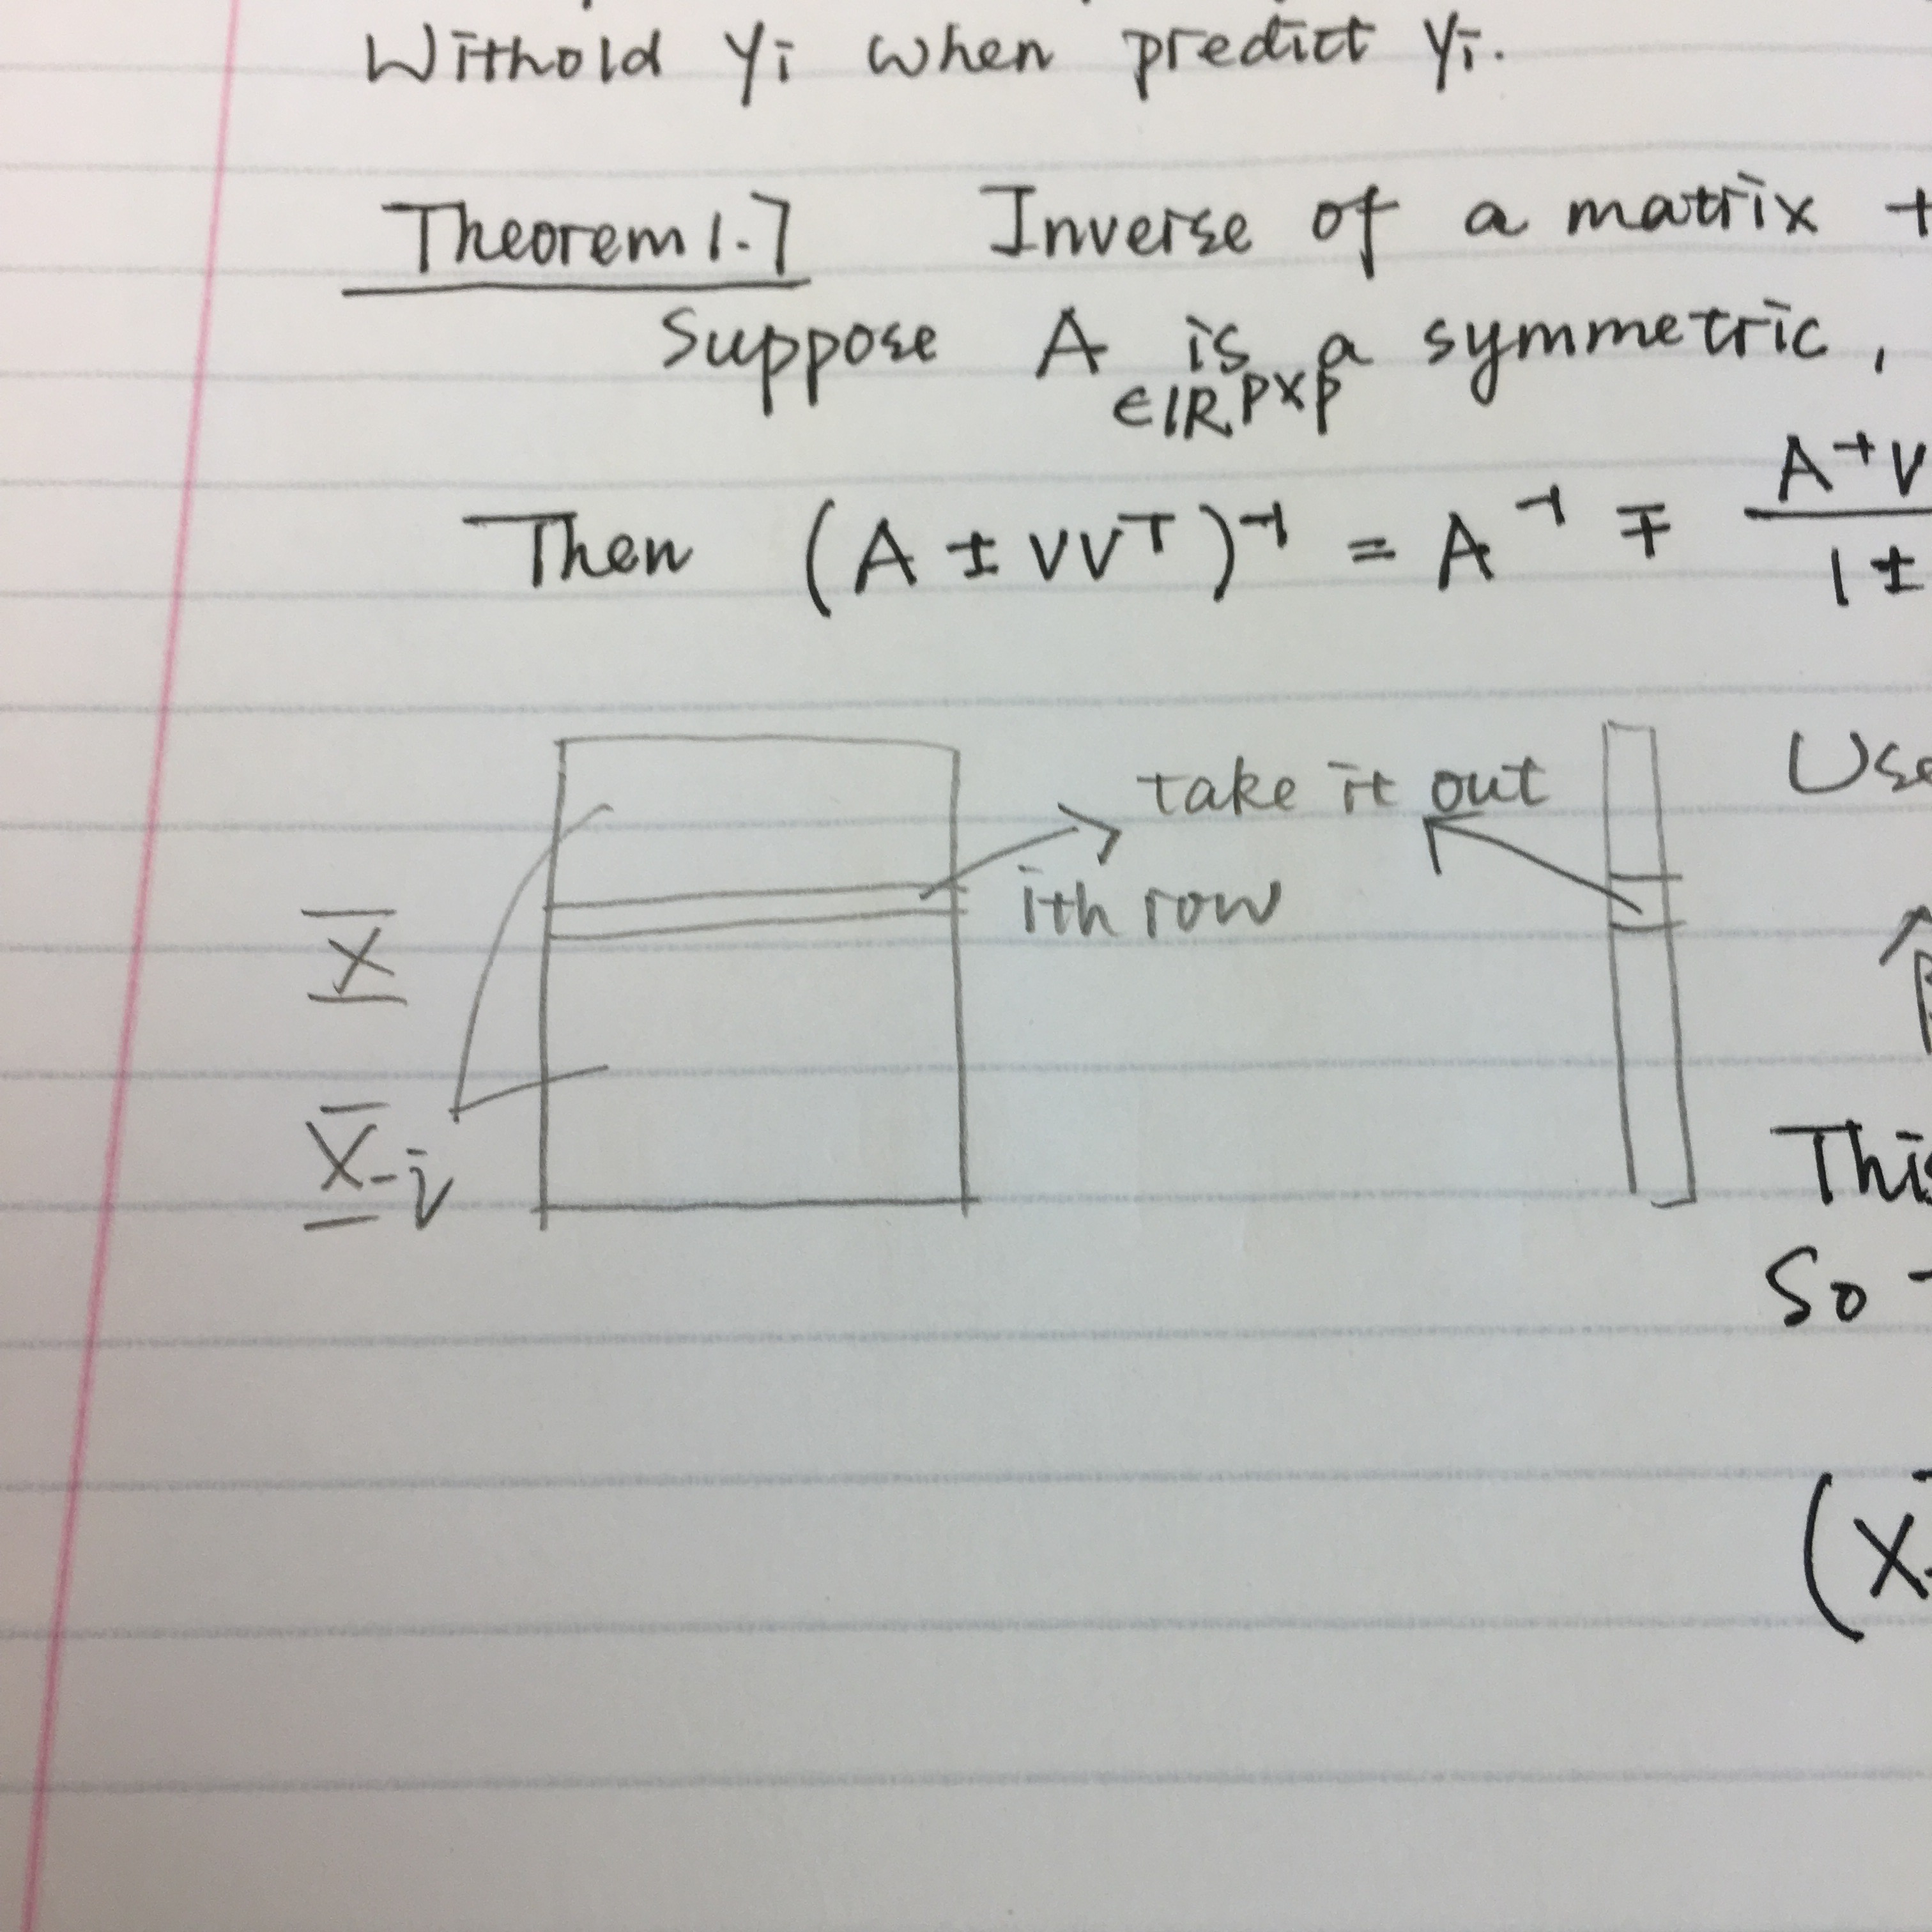
\includegraphics[scale=0.05]{wedAug31-1.jpg}
	\caption{Theorem 1.7 Visualization}
	\end{figure}

Use what is left to compute $\hat{\beta_{-i}}$.

$$\hat{\beta_{-i}} = (X^T_{-1}X_{-i})^{-1}X^T_{-i} y_{-i}$$

This can be expanded in simple sum, so that you don't have to do n regressions.

\begin{align*}
	(X^T_{-i} X_{-i})^{-1} &= (X^TX-X_iX_i^T)^{-1}\\
	&=A^{-1} + \frac{A^{-1}v v^T A^{-1}}{1 - v^t A^{-1} v}\\
	&=(X^T X)^{-1} + \frac{(X^TX)^{-1}X_i X_i^T (X^TX)^{-1}}{1 - X^T_i M X_i}\\
	X_i^T M X_i &= X_i^T (X^T X)^{-1}  \\
	&= (P_x)_{ii}\\
	&= P_i\\
	\\
	\hat{\beta}_i &= (X^TX - X_iX_i^T)^{-1} (X^T y - X_i y_i)\\
	&= [M + \frac{M X_i X_i^T M}{1 - P_i}] (X^T y - X_i y_i)\\
	&= M X^T y + \frac{M X_i X_i^T M X^T y}{1 - P_i} - M X_iy_i - \frac{M X_i X_i^T M X_i y_i}{1 - P_i}\\
	&= \dots\\
	&= \hat{\beta} - \frac{M X_i}{1 - P_i}(y_i - X_i^T \hat{\beta})
\end{align*}

Delete-one regression. 

$X_i\hat{\beta_{-i}} = \hat{y}_i - \frac{P_i}{1 - P_i} (y_i - \hat{y_i})$

\textbf{Friday September 2}\\
\\

Delete- one error

$$y_i - \hat{y}_i^{(-i)}$$

\begin{remark}
	Recall, you want to leave out $y^{i}$ so you don't overfit. 
\end{remark}


The above is equivalent to 

\begin{align*}
	y_i - X_i^T \hat{\beta}_{-i}\\
	y_i - \hat{y}_i - \frac{P_i}{1 - P_i} (y_i - \hat{y_i})\\
	(y_i - \hat{y}_i) (1 - \frac{P_i}{1 - P_i}))\\
	\frac{1}{1 - P_i} (y_i - \hat{y}_i)
\end{align*}

% GET INUITION ABOUT ABOVE

Delete-one cross validation 

$\displaystyle \sum^n_{i=1} (y_i - \hat{y}_i^{(-i)})^2$

This method is not affected by over fitting. 

The following is often used for "tuning" or variable selection (i.e. penalty, bandwidth, regularization, etc).
$ \displaystyle \sum^n_{i=1} \frac{1}{(1 - P_i)^2}(y_i - \hat{y}_i)^2$

Note: we will come back to variable selection later. 

$\beta = \begin{pmatrix} \beta_1  \\  
\vdots \\
\beta_n
 \end{pmatrix}$

$ A \subseteq \{1, \dots, P \}$

Cross validation of $A$ minimizes over $A \in 2^{\{1, \dots, P \}}$. Best cross validation set. 




\section{Residuals}\index{Residuals}

\begin{itemize}
	\item Residual
		$$\hat{e}_i = y_i - \hat{y}_i $$
	\item Standardized Residual
		$$\text{Var}(\hat{e}_i) = \text{Var}(y_i - \hat{y}_i) = \text{Var}((Q_X)_{ii}y_i)$$
		$$= ((Q_X)_{ii}y_i) \sigma^2 $$
		$$= (1 - P_i)\sigma^2 $$
		$$ sd(\hat{e}_i) = \sqrt{1-P_i} \sigma $$
		$$\hat{sd}(\hat{e}_i) = \sqrt{1-P_i} \tilde{\sigma} $$
		$$ \tilde{\sigma} = \frac{\displaystyle \sum^n_{i=1} (y_i - \hat{y}_i^{(-i)})^2}{n-p}$$
	\item Standardized residual
		$$E^*_i = \frac{\hat{e}_i}{\tilde{\sigma} \sqrt{1 - P_i}} $$
	\item Prediction Error Sum of Squares (PRESS) Residual
		$$y_i - \tilde{y}_i^{(-i)} = \frac{1}{1-P_i} \hat{e}_i = \hat{e}_{iP} $$

		$$ \hat{e}_{iP} \sim N(0, \frac{\sigma^2}{1 - P_i})$$
	\item Standardized PRESS Error
		$$\frac{\hat{e}_{iP}}{\tilde{\sigma}/ \sqrt{1-{_i}}} = \frac{\frac{1}{1-P_i}\hat{e}_i}{\tilde{\sigma}\\(\sqrt{1 - P_i})} = \frac{\hat{e}_i}{\tilde{\sigma}\\(\sqrt{1 - P_i})} = e^*_i$$
\end{itemize}

\section{Influence and Cook's Distance}\index{Influence, Cook's Distance}
% PHOTO
\begin{definition}[Influence] The difference between predictions with and without a data point.
	$$\hat{y}_i - \hat{y}_i^{(-i)} $$

\end{definition}

$$\hat{y}_i - \hat{y}_i^{(-i)} $$

$$X_i\hat{\beta} - X_i\hat{\beta}_{-i} $$

	$$\propto || X_i\hat{\beta} - X_i\hat{\beta}_{-i} ||^2	$$
	$$= (X(\hat{\beta} - \hat{\beta}_{-i}))^T (X(\hat{\beta} - \hat{\beta}_{-i})) $$
	$$(\hat{\beta} \hat{\beta}_{-i})^T X^TX (\hat{\beta} \hat{\beta}_{-i}) $$


Recall, 

$\hat{\beta}_{-i} - \hat{\beta} = -\frac{MX_i (y_i - \hat{y}_i)}{1 - P_i} = - \frac{MX_i \hat{e}_i}{1 - P_i}$

$|| X_i\hat{\beta} - X_i\hat{\beta}_{-i} ||^2 = \frac{}{} $

$= $


Cook's Distance (Technometrics, 1976?)

$$||\frac {\hat{y} - \hat{y}^{(-i)} ||^2}{\mathscr{p} \tilde{\sigma}^2} = \frac{|i \hat{e}_i^2}{(1 - P_i)^2 \mathscr{p} \tilde{\sigma}^2} $$

\begin{definition}[Cook's Distance] Cook's distance measures the influence of the $i^{th}$ deservation.
\end{definition}

\section{Orthogonal Decomposition}\index{Orthogonal Decomposition}

Recall,
$\mathbb{R}^n$ is Euclidean Space.\\

$\mathscr{S}$ is a subspace ($\mathscr{S} \leq \mathbb{R}^n$)

\begin{remark}
	$\leq$ is subspace\\
	$\subseteq$ is a subset
\end{remark}

For 

$\mathscr{S}_1 \leq \mathscr{S}_1 \mathscr{S}_2 \leq \mathscr{S}$

$$\mathscr{S}_1 + \mathscr{S}_2 = \{x + y: x \in \mathscr{S}_1, y \in \mathscr{S}_2 \} $$

% PHOTO

Suppose $\mathscr{S}_1, \mathscr{S}_2 \leq \mathscr{S}$, 

$\mathscr{S}_1 + \mathscr{S}_2 = \mathscr{S}$, $\mathscr{S}_1 \perp \mathscr{S}_2$

then, 

	$$\{\mathscr{S}_1, \mathscr{S}_2 \} $$ is called an orthogonal decomposition of $\mathscr{S}$

% PHOTO

In this case, 

	$$\mathscr{S}_1 \oplus \mathscr{S}_2 = \mathscr{S} $$

More generally, 

\begin{definition}[Orthogonal Decompositon (O.D.)]
	Let $\mathscr{S}_1, \dots, \mathscr{S}_k$ be subspaces of $\mathscr{S}$ such that

	\begin{enumerate}
		\item $\mathscr{S}_1, \dots, \mathscr{S}_k = \{v_1 + \dots + v_k : v_1 \in \mathscr{S}_1, \dots, v_k \in \mathscr{S}_k\}$
		\item $\mathscr{S}_i \perp \mathscr{S}_j \quad \forall i\neq j$
	\end{enumerate}
	
	Then, $\{\mathscr{S}_1, \mathscr{S}_2, \dots, \mathscr{S}_k\}$ is an \textbf{orthogonal decomposition} of $\mathscr{S}$. We may write $\mathscr{S} = \mathscr{S}_1 \oplus \mathscr{S}_2 \oplus \dots \oplus \mathscr{S}_k$.
\end{definition}

\textbf{Proposition 1.5} If $\mathscr{S}_1, \dots, \mathscr{S}_k$ is an O.D. of $\mathscr{S}$, then any $v \in \mathscr{S}$ can be uniquely written as

$$v_1 + \dots + v_k$$, where $v_1 \in \mathscr{S}_1, \dots v_k \in \mathscr{S}_k$. \\

\textbf{Wednesday September 7}

\begin{definition}[Direct Difference]
	Let $\mathscr{S}_1 \leq \mathscr{S}_2 \leq \mathbb{R}^n$. Then, \\

	$$\mathscr{S}_2 \cap \mathscr{S}_1^\perp \equiv \mathscr{S}_2 \ominus \mathscr{S}_1 $$ 

	is called \textbf{direct difference}. This is almost the same as orthogonal complement, except it is within $\mathscr{S}_2$. 

\end{definition}

\textbf{Proposition 1.6} If $\mathscr{S}_1 \leq \mathscr{S}_2$, then 

$$\mathscr{S}_2 = \mathscr{S}_1 \oplus (\mathscr{S}_2 \ominus \mathscr{S}_1) $$

\textbf{Proposition 1.7 - Orthogonal Decomposition and Projection} Consider a Hilbert Space, $\mathscr{H} = \{\mathbb{R}^n, <,>_A \}$, 

\begin{enumerate}
	\item If $\mathscr{S} \leq \mathscr{S}_1 \perp \mathscr{S}_2$ in $\mathscr{H}$, then 

	$$P_{\mathscr{S}_1} (A) P_{\mathscr{S}_2} (A) = 0  $$

	\item If $\mathscr{S} \leq \mathscr{H}, \dots, \mathscr{S}_k \leq \mathscr{H}$, and $\mathscr{S}_1 \perp \dots \perp \mathscr{S}_k$, then

	$$P_{\mathscr{S}_1, \oplus \dots \oplus \mathscr{S}_k} (A) = P_{\mathscr{S}_1} (A) + \dots + P_{\mathscr{S}_k} (A) $$

	\item If $\mathscr{S}_1 \leq \mathscr{S}_2 \leq \mathbb{R}^n$, then

	$$P_{\mathscr{S}_2 \ominus \mathscr{S}_1} (A) = P_{\mathscr{S}_2} (A) - P_{\mathscr{S}_1} (A)$$
\end{enumerate}


\begin{theorem}[Generalization of the earlier Cochran's Theorem]

Suppose $X \sim N(0, \Sigma)$ where $\Sigma \in \mathbb{R}^{nxn}$ is positive definite. 

Let $\mathscr{H} = \{ <,>_{\Sigma^{-1}}\}$. Suppose $\mathscr{S}_1, \dots \mathscr{S}_k, \mathscr{S} \leq \mathscr{H}$ such that $\mathscr{S} = \mathscr{S}_1 \oplus \dots \oplus \mathscr{S}_k$.\\

Let 

	$$w_i = ||P_{\mathscr{S}_i} (\Sigma^{-1}) X ||^2_{\Sigma^{-1}} $$
	$$w = ||P_{\mathscr{S}} (\Sigma^{-1}) X ||^2_{\Sigma^{-1}} $$

Then, 

\begin{enumerate}
	\item $ w = w_1 + \dots + w_k$
	\item $ w_1 \indep \dots \indep w_k$
	\item $w_i \sim \chi^2_{r_i}$\\
		$w \sim \chi^2_{r}$\\
		where $r_i$ is the $dim(\mathscr{S}_i)$, $r$ is the $dim(\mathscr{S})$, and $r = r_1 + \dots + r_k$.
\end{enumerate}
	
\end{theorem}

\begin{notation}
	We use $\oplus$ for spaces. We can also use $\oplus$ function to stack up matrices. Let $A_1, \dots, A_k$ be matrices with arbitrary dimensions. 

	$$A_1 \oplus \dots \oplus A_k = \begin{pmatrix}
		A_1 & \dots & 0\\
		    & \ddots & \\
		0 & \dots & A_k
	\end{pmatrix} $$
\end{notation}

\section{Lack of Fit Test}\index{Lack of Fit Test}

Goodness of Fit

% GET PHOTO

At each $x_i$ you have multiple observations, say $y_{i1}, \dots, y_{im_i}$. In this case, you may test to see if a linear model,$y_i = x_i^T \beta + \epsilon_i$ , is the correct choice for fitting the data. In general, lack of fit refers to testing whether any (linear, generalized, etc) model is adequately describing the data. 

Denote 

$y_i = \begin{pmatrix}
	y_{i1}\\
	\vdots\\
	y_{im_i}
\end{pmatrix}$

$1_{m_i} = \begin{pmatrix}
	1 \\
	\vdots\\
	1
\end{pmatrix}$

$X = \begin{pmatrix}
	X_{1}^T\\
	\vdots\\
	X_{m}^T
\end{pmatrix}$

Assume

$$y_{ij} = X_i^T \beta + \epsilon_{ij} $$

where $\epsilon \sim^{iid} N(0, \sigma^2)$. 

The point is that you have $y_{i1} \dots y_{jm}$ for each $X_i$.\\

In matrix form, 

% GET PHOTO

$$(1_{m_1} \oplus \dots \oplus 1_{m_n}) X\beta + \epsilon $$

So, let $N$ denote a full sample size. 

$$N = m_1 + \dots + m_n$$

this is a special case of linear model, except the design matrix is structured $(1_{m_1} \oplus \dots \oplus 1_{m_n})X $ instead of X. So the formula for MLE (and so on) is the same. \\

$$X \leftrightarrow (1_{m_1} \oplus \dots \oplus 1_{m_n})X$$

So, 

$$\hat{\beta} = ([(1_{m_1} \oplus \dots \oplus 1_{m_n})X])^T ([(1_{m_1} \oplus \dots \oplus 1_{m_n})X])^{-1} [(1_{m_1} \oplus \dots \oplus 1_{m_n})X]^T y$$

\begin{align*}
\hat{y} &= (1_{m_1} \oplus \dots \oplus 1_{m_n})X \hat{\beta} \\
	&= (1_{m_1} \oplus \dots \oplus 1_{m_n})X ([(1_{m_1} \oplus \dots \oplus 1_{m_n})X])^T ([(1_{m_1} \oplus \dots \oplus 1_{m_n})X])^{-1} [(1_{m_1} \oplus \dots \oplus 1_{m_n})X]^T y\\
	&=  (1_{m_1} \oplus \dots \oplus 1_{m_n})X [X^T \begin{pmatrix}
		m_1 & \dots & 0\\
		  & \ddots  & \\
		  0 & \dots & m_n
	\end{pmatrix} 	X]^{-1} X^T (1_{m_1} \oplus \dots \oplus 1_{m_n})	
\end{align*}

So, in linear model with replication we have our hypotheses for lack of fit test, 

$$H_O: E(y_i) = 1_{m_i} X_i^T \beta$$
$$H_1: E(y_i) = 1_{m_i} \mu_i $$

% GET PHOTO 

We are testing whether the arbitrary means, $\mu_1, \dots \mu_n$ sit on the same line. \\


\textbf{Friday September 9}

Under $H_1$, 

$$ y = (1_{m_1} \oplus \dots \oplus 1_{m_n}) \begin{pmatrix}
	\mu_1\\
	\vdots\\
	\mu_n
\end{pmatrix}
+ \epsilon$$

So the $\hat{y}$ under this model, 

$$\hat{y}_{H_1} = P_{1_{m_1} \oplus \dots \oplus 1_{m_n}} y = (1_{m_1} \oplus \dots \oplus 1_{m_n}) \begin{pmatrix}
	m_1 & & \\
	 & \ddots & \\
	  &  & m_n
\end{pmatrix} (1_{m_1} \oplus \dots \oplus 1_{m_n})^T y$$

but under $H_0$, 

$$ \hat{y}_{H_0} = P_{(1_{m_1} \oplus \dots \oplus 1_{m_n})X} y$$

$$\mathscr{S}_1 = \text{span}\{(1_{m_1} \oplus \dots \oplus 1_{m_n})X \} \quad \text{(p-dim)}$$

$$\mathscr{S}_2 = \text{span}\{(1_{m_1} \oplus \dots \oplus 1_{m_n}) \} \quad \text{(n-dim)}$$

$$\mathscr{S}_3 = \mathbb{R}^N \quad (N = m_1 + \dots + m_n)$$

$$ \mathscr{S}_1 \leq \mathscr{S}_2 \leq \mathscr{S}_3 $$

\begin{remark}
	Above used the fact that span(AB) $\subseteq$ span(A)
\end{remark}

\textbf{Lemma 1.1} If $ \mathscr{S}_1 \leq \mathscr{S}_2 \leq \mathscr{S}_3$ then

\begin{enumerate}
	\item $\mathscr{S}_3 \ominus \mathscr{S}_2 \leq \mathscr{S}_3 \ominus \mathscr{S}_1$		  \item $(\mathscr{S}_3 \ominus \mathscr{S}_1) \ominus \mathscr{S}_2 =  \mathscr{S}_3 \mathscr{S}_2$
	\item $(\mathscr{S}_3 \ominus \mathscr{S}_1) = (\mathscr{S}_3 \ominus \mathscr{S}_2) \oplus (\mathscr{S}_2 \ominus \mathscr{S}_1)$
 
\end{enumerate}

Go back to lack of fit, 

$$(\mathscr{S}_3 \ominus \mathscr{S}_1) = (\mathscr{S}_3 \ominus \mathscr{S}_2) \oplus (\mathscr{S}_2 \oplus \mathscr{S}_1)$$

$$P_{\mathscr{S}_3 \ominus \mathscr{S}_1}y = P_{\mathscr{S}_3 \ominus \mathscr{S}_3}y + P_{\mathscr{S}_2 \ominus \mathscr{S}_1}y \quad \text{(Orthogonal Decomposition)} $$

$$||P_{\mathscr{S}_3 \ominus \mathscr{S}_1}y||^2 = ||P_{\mathscr{S}_3 \ominus \mathscr{S}_3}y||^2 + ||P_{\mathscr{S}_2 \ominus \mathscr{S}_1}y||^2 $$

$$dim(\mathscr{S}_2 \ominus \mathscr{S}_1) = n-p$$

$$dim(\mathscr{S}_3 \ominus \mathscr{S}_2) = N-n$$

Now, 

$$E(P_{\mathscr{S}_3 \ominus \mathscr{S}_2}y) = P_{\mathscr{S}_3 \ominus \mathscr{S}_2}E(y) =P_{\mathscr{S}_3 \ominus \mathscr{S}_2} \mu  = 0 $$

But, 

$\mu = \begin{pmatrix}
	\mu_1\\
	\vdots\\
	\mu_n
\end{pmatrix} \in \mathscr{S}_2$

and, 

$(1_{m_1} \oplus \dots \oplus 1_{m_n})\underline{\mu}$

$$Var(P_{\mathscr{S}_3 \ominus \mathscr{S}_2}y) = P_{\mathscr{S}_3 \ominus \mathscr{S}_2}Var(y)P_{\mathscr{S}_3 \ominus \mathscr{S}_2} = \sigma^2 P^2_{\mathscr{S}_3 \ominus \mathscr{S}_2} = \sigma^2 P_{\mathscr{S}_3 \ominus \mathscr{S}_2} $$

We know that $y \sim N(\mu, \sigma^2 I_n)$. So, 

$$P_{\mathscr{S}_3 \ominus \mathscr{S}_2}y \sim N(0, \sigma^2 P_{\mathscr{S}_3 \ominus \mathscr{S}_2} $$

Similarly, 

$$ E(P_{\mathscr{S}_2 \ominus \mathscr{S}_1}y) = P_{\mathscr{S}_2 \ominus \mathscr{S}_1}E(y)$$

which under $H_0$ is, 

$$P_{\mathscr{S}_2 \ominus \mathscr{S}_1} (1_{m_1} \oplus \dots \oplus 1_{m_n})X\beta = 0 $$

$$Var(P_{\mathscr{S}_2 \ominus \mathscr{S}_1}y) = \sigma^2 P_{\mathscr{S}_2 \ominus \mathscr{S}_1} $$

$$P_{\mathscr{S}_2 \ominus \mathscr{S}_1} y \sim N(0, \sigma^2 P_{\mathscr{S}_2 \ominus \mathscr{S}_1})$$

By Chochran's Theorem: 

	Under $H_O$, 

	$$||P_{\mathscr{S}_3 \ominus \mathscr{S}_2} y||^2 \sim \chi^2_{(N-n)} $$
	$$||P_{\mathscr{S}_2 \ominus \mathscr{S}_1} y||^2 \sim \chi^2_{(n-p)} $$

	$$||P_{\mathscr{S}_3 \ominus \mathscr{S}_2} y||^2 \indep  ||P_{\mathscr{S}_2 \ominus \mathscr{S}_1} y||^2$$

So our lack of fit test is: 

	$$\frac{||P_{\mathscr{S}_2 \ominus \mathscr{S}_1} y||^2 / (n-p)}{||P_{\mathscr{S}_3 \ominus \mathscr{S}_2} y||^2 / (N - n)} \sim F _{n-p, N-n} $$



 \section{Explicit Intercept}\index{Explicit Intercept}


We now apply this $\mathscr{S}_1, dots $ argument to another problem: special linear model. 

$$y_i = \alpha + \beta^TX_i + \epsilon_i 	\quad i = 1, \dots, n $$

$y = \begin{pmatrix}
	y_1\\
	\vdots\\
	y_n
\end{pmatrix}$

$X = \begin{pmatrix}
	X_1\\
	\vdots\\
	X_n
\end{pmatrix}$

$\epsilon = \begin{pmatrix}
	\epsilon_1\\
	\vdots\\
	\epsilon_n
\end{pmatrix}$

$$Y = 1_n \alpha + X\beta + \epsilon = (1_n X)\begin{pmatrix}
	\alpha\\
	\beta
\end{pmatrix} + \epsilon = U\eta + \epsilon$$

Let $P_{1_n} = 1_n(1_n^T 1_n)^{-1} 1_n^T = \frac{1_n1_n^T}{n}$.\\

Note that for all $a = \begin{pmatrix}
	a_1\\
	\vdots\\
	a_n
\end{pmatrix} \in \mathbb{R}^n$, 

	$$P_{1_n}a = \frac{1_n 1_n^T a}{n} = 1_n \bar{a}, \quad \bar{a}= \frac{1}{n}\displaystyle\sum^n_{i=1}a_i $$

	which is a mean projection. (?)

	$Q_{1_n} = I_n - P_{1_n} \quad \text{(projection on}1_n^\perp\text{)}$\\

	$$ Q_{1_n} a = \begin{pmatrix}
		a_1 - \bar{a}\\
		\vdots \\
		a_n - \bar{a}

	\end{pmatrix}$$

	Decompose X:

	$$X = P_{1_n}X + Q_{1_n}X $$

	$$U \eta = 1_n \alpha + X\beta = 1_n \alpha + P_{1_n}X\beta + Q_{1_n}X\beta = 1_n (\alpha + \frac{1_n^T X\beta}{n}) + Q_{1_n}X\beta = (1_n Q_{1_n}X)\begin{pmatrix}
		\alpha^\star\\
		\beta
	\end{pmatrix} = (1_n Q_{1_n}X)\eta^\star = U^\star\eta^\star $$

	So we do least squres of

	$$(y - U^\star\eta^\star)^T(y - U^\star\eta^\star)$$

	and minimize this over all $\eta^\star \in \mathbb{R}^{Px1}$


	$$\hat{\eta}^\star = (U^{\star T} U^\star)U^{\star T} y $$

	$$U^{\star T} U^\star = \begin{pmatrix}
		1_n^T\\
		(Q_{1_n}X)^T
	\end{pmatrix} (1_n Q_{1_n}X) = \begin{pmatrix}
		1_n^t1_n & Q_{1_n}X1_n\\
		1_n^TQ_{1_n}X & Q_{1_n}X Q_{1_n}X\\
	\end{pmatrix}  = \begin{pmatrix}
		n & 0 \\
		0 & X^TQ_{1_n}X
	\end{pmatrix}$$

	$$\hat{\eta}^\star = \begin{pmatrix}
		n^{-1} & 0 \\
		0 & (X^T Q_{1_n}X)^{-1}
	\end{pmatrix} \begin{pmatrix}
		1_n \\
		(Q_{1_n}X)^T
	\end{pmatrix} y$$

	\textbf{Monday September 12}

	So 

	$$\hat{\alpha}^\star = n^{-1}1_n^T y $$

	$$\hat{\beta} = (X^TQX)^{-1} X^TQ y $$

	$$\hat{\alpha} = n^{-1} 1^T_n y - n^{-1}X \hat{\beta}^\star $$

	For statistical inference, we want to make a decomposition of $\mathbb{R}^n$.

	Let, $\mathscr{S}_1 = \text{span}(1_n), \mathscr{S}_2 = \text{span}(1_n, X), \mathscr{S}_3 = \mathbb{R}^n$. \\

	Then,

	$$(\mathscr{S}_3 \ominus \mathscr{S}_1) = (\mathscr{S}_3 \ominus \mathscr{S}_2) \oplus (\mathscr{S}_2 \ominus \mathscr{S}_1) $$

	Then, 

	$$||P_{\mathscr{S}_3 \ominus \mathscr{S}_1}y||^2 = ||P_{\mathscr{S}_3 \ominus \mathscr{S}_2}y||^2 + ||P_{\mathscr{S}_2 \ominus \mathscr{S}_1}y||^2 $$

	Or, 

	$$SSTotal = SSError + SSRegression $$ 

	We may compute these terms, 

	\begin{align*}
		P_{\mathscr{S}_3 \ominus \mathscr{S}_1} =  P_{\mathscr{S}_3} - P_{\mathscr{S}_1}\\
			&= I_n - \frac{1_n1_n}{1_n^T1_n}\\
			&= Q_1n\\
		\mathscr{S}_2 \ominus \mathscr{S}_1	&= \text{span}(Q_{1_n}X)\\
		P_{\mathscr{S}_2 \ominus \mathscr{S}_1} &= QX(X^TQX)^{-1}QX^T\\
		P_{\mathscr{S}_3 \ominus \mathscr{S}_2}&= Q - QX(X^TQX)^{-1}X^TQ
	\end{align*}

By Cochran's Theorem, (these are orthogonalized projections, etc), 

$$ ||P_{\mathscr{S}_3 \ominus \mathscr{S}_1}y||^2 \sim \chi^2{(n-1)} $$
$$ ||P_{\mathscr{S}_2 \ominus \mathscr{S}_1}y||^2 \sim \chi^2_{(p-1)} $$
$$ ||P_{\mathscr{S}_3 \ominus \mathscr{S}_2}y||^2 \sim \chi^2_{(n - p - 1)} $$

\begin{remark}
	$$dim(\mathscr{S}_3) = n$$
	$dim(\mathscr{S}_2) = p+1$
	$dim(\mathscr{S}_3) = 1$
\end{remark}

We also know that these are all independent of each other. So we can test regression effect with the following hypothesis:

$$H_0: \beta - 0 $$


$$\frac{||P_{\mathscr{S}_2 \ominus \mathscr{S}_1}y||^2 / (p-1)}{||P_{\mathscr{S}_3 \ominus \mathscr{S}_2}y||^2 / (n-p - 1)} = \frac{y^T QX(X^TQX)^{-1}QX^T y /(p-1)}{y^T (Q - QX(X^TQX)^{-1}X^TQ) y / (n-p - 1)} \sim F_{p-1, n - p - 1} $$

Distributions\\

$$\hat{\beta} (X^TQX)^{-1}X^TQy$$

$E(\hat{\beta}) = (X^TQX)^{-1}X^TQ(1_{n\alpha} + X\beta = (X^TQX)^{-1}X^TQX \beta = \beta$

$\text{Var}(\hat{\beta}) =  (X^TQX)^{-1}X^TQ (\sigma^2 I_n) QX (X^TQX)^{-1} = \sigma^s(X^TQX)^{-1} $

$\hat{\alpha} = \hat{\alpha}^\star - X^T \hat{\beta}$

Because $\hat{\beta}$ is a function of $Qy$ and $\hat{\alpha}^\star$ is a function of $P_{1_n}y$ (and these are orthogonal to each other and thus by normality also independent). \\

$\text{Var}(\hat{\alpha} = \text{Var}(\hat{\alpha}^\star) + \text{Var}( \bar{X}^T \hat{\beta}) = \text{Var}(\bar{y}) + \text{Var}( \bar{X}^T \hat{\beta}) = \frac{\sigma^2}{n} + \sigma^2 \bar{X}^T(X^TQX)^{-1} \bar{X} $

$$\hat{\alpha} ~ N( \alpha, \frac{\sigma^2}{n} + \sigma^2 \bar{X}^T(X^TQX)^{-1} \bar{X}) $$

\begin{align*}
	Cov(\hat{\alpha}, \hat{\beta}) &= Cov(\hat{\alpha}^\star - \bar{X}^T\hat{\beta}, \hat{\beta})\\
		&=-\bar{X}^T Var(\hat{\beta})\\
		&= =\bar{X}^T \sigma^2 (X^TQX)^{-1}
\end{align*}

$$ \begin{pmatrix}
	\hat{alpha}\\
	\hat{\beta}
\end{pmatrix} \sim N[\begin{pmatrix}
	\alpha\\
	\beta
\end{pmatrix}, \begin{pmatrix}
	\frac{\sigma^2}{n} + \sigma^2 \bar{X}^T(X^TQX)^{-1} \bar{X} & - \sigma^2 \bar{X}^T(X^TQX)^{-1} \bar{X}\\
	- \sigma^2 \bar{X}^T(X^TQX)^{-1} \bar{X} & \frac{\sigma^2}{n} + \sigma^2 \bar{X}^T(X^TQX)^{-1} \bar{X}
\end{pmatrix}]$$

Estimate $\sigma^2$\\


$$ ||P_{\mathscr{S}_3 \ominus \mathscr{S}_2}y||^2 = \displaystyle \sum^n_{i=1} (y_i - \hat{\alpha} - \hat{\beta}^TX_i)^2 \sim \sigma^2 \chi^1_{n-p-1}$$

So, 

$$E(||P_{\mathscr{S}_3 \ominus \mathscr{S}_2}y||^2 ) = \sigma^2 (n-p-1)$$

Thus, 

$$\hat{\sigma}^2 = \frac{||P_{\mathscr{S}_3 \ominus \mathscr{S}_2}y||^2 }{n-p-1}$$

\begin{theorem}
	Under the explicit intercept model, 

	\begin{enumerate}
		\item $(\hat{\alpha}, \hat{\beta}, \hat{\sigma}^1)$ is UMVUE of $(\alpha, \beta, \sigma^2)$ by Lehmann-Sheffe.
		\item $$ \begin{pmatrix}
	\hat{\alpha}\\
	\hat{\beta}
\end{pmatrix} \sim N[\begin{pmatrix}
	\alpha\\
	\beta
\end{pmatrix}, \begin{pmatrix}
	\frac{\sigma^2}{n} + \sigma^2 \bar{X}^T(X^TQX)^{-1} \bar{X} & - \sigma^2 \bar{X}^T(X^TQX)^{-1} \bar{X}\\
	- \sigma^2 \bar{X}^T(X^TQX)^{-1} \bar{X} & \frac{\sigma^2}{n} + \sigma^2 \bar{X}^T(X^TQX)^{-1} \bar{X}
\end{pmatrix}]$$
	\item $(n-p-1) \hat{\sigma}^2 \sim \sigma^2 \chi^2_{(n-p-1)}$
	\item $\begin{pmatrix}
			\hat{\alpha}\\
			\hat{\beta}
		\end{pmatrix} \indep \hat{\sigma}^2$
	\end{enumerate}
\end{theorem}



% %------------------------------------------------




\section{$R^2$}\index{$R^2$}

Proportion of Sum of Squares (SS) explained by regression (i.e. by $\beta$). 

$$R^2 = \frac{SSR}{SST} = \frac{||P_{\mathscr{S}_2 \ominus \mathscr{S}_1}y||^2}{||P_{\mathscr{S}_3 \ominus \mathscr{S}_1}y||^2}$$

But we know that, 

$$R^2 = \frac{||P_{\mathscr{S}_2 \ominus \mathscr{S}_1}y||^2}{||P_{\mathscr{S}_2 \ominus \mathscr{S}_1}y||^2 + ||P_{\mathscr{S}_3 \ominus \mathscr{S}_2}y||^2} = \frac{SSR}{SSR + SSE} = \frac{SSR/SSE}{SSR/SSE + 1} $$

$$ F = \frac{SSR/p}{SSE/(n-p-1)} = \frac{(n-p-1)}{p} \frac{SSR}{SSE} $$

$$ \frac{SSR}{SSE} = \frac{p}{(n-p-1)} F$$

$$R^2 = \frac{\alpha F}{\alpha F - 1}$$
where $\alpha = \frac{p}{n-p-1}$

This is how we compute the null distribution of $R^2$. \\

\section{Multicollinearity}\index{Multicollinearity}

\textbf{Wednesday September 14}\\

$y = C_1 \beta_1 + \dots + C_p \beta_p$

$$ X = (C_1, \dots, C_P) = \begin{matrix}
	X^T_1\\
	\vdots\\
	X^T_n
\end{matrix}$$

In an extreme case, multicolinearity simply means that the $C_1, \dots, C_p$ are linearly dependent. In this case $\beta$ is not identifiable. 

	We have $C_1, C_2, C_3$.\\

	\begin{align*}
		C_1 &= a\\
		C_2 &= 2a\\
		C_3 &= b
	\end{align*}

	\begin{align*}
		y &= a\beta_1 + 2a \beta_2 + b\beta_3 + \epsilon\\
		&= a(\beta_1 + 2\beta_2) + b\beta_3 + \epsilon
	\end{align*}
	
	$\beta_1 \& \beta_2$ cannot be split. \\

	In the less extreme case, $X^TX$ is nearly singular, meaning it has small eigenvalues. In this case, although $\beta$ is identifiable, they have large variance For example, if $C_1 = a C_2 x 2a$ then $\beta_1, \beta_2$ have large variance which means your parameterization is not good. So may define new parameterization.

	$$ \gamma_1 = \beta_1 + 2\beta_2$$
	$$ \gamma_2 = \beta_3$$ 

	If you run regression against these then the variance would be 'normal'.\\

	S0, how to wee out redundant varaibles? One way Variance Inflation Factor (VIF) which for each $ i = 1, 2, \dots, p$ regresses $C_i$ on $\{C_1, \dots, C_p \setminus C_i \}$
then you get $R^2$ for this regression call it $R_i^2$.\\

If $C_i$ is redunent then $R_i^2$ would be close to 1. 

$$VIF_i = \frac{1}{1 - R_i^2} $$





% %------------------------------------------------





\section{Variable Selection}\index{Variable Selection}

$$ y = C_1\beta_1 + \dots + C_p\beta_p + \epsilon$$

Some of these $\beta$'s are zero. \\

Let us define an active set of parameters, 

$$A_0 = \{i: \beta_i \neq 0 \}$$

To estimate $A_0$ is the goal of variable selction. \\

\textbf{Mallow's $C_p$ criterion}\\

The fundamental issue is variable selction, penalty - penalizing the number of parameters, so you cannot use something like $y - \hat{y}$ as criterion. The more variables you have the smaller $||\hat{y} - y ||^2$ is. So we want to penalize the number of parameters in a reasonable way. \\

Let any subset $A \subset \{1, \dots, p\}$, 

$$X_A = \{C_i: i \in A \}$$

\begin{notation}
	While we often use X  for iid variables (a vector), but here X is a matrix and $X_i$ were referring to its columns. We've changed $X_i$ to $C_i$ to better reflect that we are dealing with columns of X. 
\end{notation}

So, $A = \{1, 3, 5\}$, 

$$X_A = \begin{pmatrix}
	C_1\\
	C_3\\
	C_5
\end{pmatrix}$$

Let $P_{X_A}, Q_{X_A}$ be the projection on to span($X_A$), span$(X_A)^\perp$. For example, 

$$P_{X_A} = X_A(X_A^T X_A)^{-1}X_A^T $$

Let $\mu = E(y) = X\beta = X_{A_0}\beta_{A_0}$.\\

\textbf{Mallow} says we minimize

$$\frac{E||P_{A}y - \mu ||^2}{\sigma^2} $$

among all $A \subset \{1, \dots, p \}$.\\

But we do not know what $\sigma^2$ or $\mu$ are. If so, we would already know $A_0$. We must estimate these.\\

$$E || P_{X_A} y - \mu ||^2 = tr(E(P_{X_A} y - \mu)(P_{X_A} y - \mu)^T) $$

\begin{align*}
	E(P_{X_A} y - \mu)(P_{X_A} y - \mu)^T &= E[(P_{X_a}y - P_{X_a}\mu) + (P_{X_a}\mu - \mu)][(P_{X_a}y - \mu)+ (P_{X_a}\mu - \mu)]^T\\
		&=  \text{expand, two terms are zero}\\
		&= E(P_{X_a}y - P_{X_a}\mu)(P_{X_a}y - P_{X_a}\mu) + (P_{X_a}\mu  - \mu)(\P_{X_a}\mu - \mu)^T\\
		&= Var(P_{X_a}y)\\
		&= P_{X_a} \sigma^2 I_n P_{X_a} = \sigma^2 P_{X_a}\\
		&= tr(\sigma^2 P_{X_a} + Q_{X_a}\mu\mu^TQ_{X_a})\\
		&= \sigma*2 tr(P_{X_a}) + tr(Q_{X_a}\mu\mu^tQ_{X_a})\\
		&= \sigma^2(\#(A)) + tr(\mu^T Q_{X_a} \mu)\\
\end{align*}

$$\Rightarrow E\frac{ || P_{X_A} y - \mu ||^2}{\sigma^2} = \#(A) + \frac{tr(\mu^T Q_{X_a} \mu)}{\sigma^2}$$

Now let's estimate $\frac{\mu^T Q_{X_a} \mu}{\sigma^2}$. \\

Recall, if $U$ is a random vector with multivariate normal distribution so

$$E(U) = e $$
$$Var(U) = Q_{X_A} $$

$$U^TU \sim \chi^2_{(rank(Q)_{X_A})} (||e||^2) $$

Also, $W \sim \chi^2_{(r)} (\delta)$ where $E(W) = r + \delta$.\\

Go back to our problem of estimating $\frac{\mu^T Q_{X_a} \mu}{\sigma^2}$. \\

What about $y^t Q_{X_A} y$? We know that

$$E (\frac{Q_{X_A}y}{\sigma}) = \frac{Q_{X_A}\mu}{\sigma}$$

and

$$Var(\frac{Q_{X_A}y}{\sigma}) = \frac{1}{\sigma^2} Q_{X_A}\sigma^2 I_n = 0$$

So, 

$$ \frac{Q_{X_A}y}{\sigma} \sim N( \frac{Q_{X_A}\mu}{\sigma}, 0)$$

So

$$(\frac{Q_{X_A}y}{\sigma})^T(\frac{Q_{X_A}y}{\sigma}) \sim \chi^2_{(n-\#(A))} ((\frac{Q_{X_A}\mu}{\sigma})^T(\frac{Q_{X_A}\mu}{\sigma})) = \chi^2_{(n-\#(A))} (\frac{\mu^T Q_{X_A} \mu}{\sigma^2}) $$

Thus, 

$$E(\frac{y^T Q_{X_A} y}{\sigma^2} ) = n - \#(A) + \frac{\mu^T Q_{X_A} \mu}{\sigma^2} $$

Which, if you subtract over the n and \#(A) you get an unbiased estimator of $\frac{\mu^T Q_{X_A} \mu}{\sigma^2}$.

But $\sigma^2$ is still unkown, but we use full model, 

$$\hat{\sigma}^2 = \frac{y^T Q_{X_A} y}{n - p} $$

Now we can estimate $\frac{\mu^T Q_{X_A} \mu}{\sigma^2} $ by 

$$\frac{y^T Q_{X_A} y}{\frac{y^T Q_{X} y}{n-p}} - n + 2\#(A) = (n-p) \frac{y^T Q_{X_A} y}{y^T Q_{X} y} - n + 2 \#(A)$$ 

So to recap,
 $$ E\frac{ || P_{X_A} y - \mu ||^2}{\sigma^2} = (n-p)\frac{y^T Q_{X_A} y}{y^T Q_{X} y} - n + 2 \#(A) $$


\textbf{Friday September 16}\\


\textbf{Akaike/Bayesian Information Criteria (AIC/BIC)}\\

Suppose we have some generic (i.e. not related to the design/covariance in regression context) $X_1, \dots, X_n$, a sample of independent random vectors with joint density $f_\theta (x_1, \dots, x_n)$.\\

$\theta \in \Theta \subset \mathbb{R}^P$\\

$\theta = \begin{pmatrix}
	\theta_1\\
	\vdots\\
	\theta_P
\end{pmatrix}$\\

Let $M_0 \subset \{1, \dots, P \}$ be the true active set, that is $\{i: \theta_i \neq 0 \} = M_0$. Also, let $M_0 \subset \{1, \dots, P\}$. We want to recover the true active set $M_0$.\\

Let $\Theta_M$ be the paramter space, corresponding to M. 

$$\Theta_M = \{\theta \in \Theta: \theta_i = 0 iff i \notin M \}$$

Of course we also thave $\Theta_{M_0}$.\\

for each $M \subset \{1, \dots, P \}$ define,

$$L_M = \sup_{\theta \in M} f_\theta (x_1, \dots, x_n) $$

Then, 

$$\text{AIC}(M) = -2 \log L_M + 2(\#M) $$

$$\text{BIC}(M) = -2 \log L_M + (\log n)(\#M) $$

Use them 

$$\hat{M} = \arg\min \{\text{AIC}(M): M \in 2^{\{1, \dots, P\}}\}$$
$$\hat{M} = \arg\min \{\text{BIC}(M): M \in 2^{\{1, \dots, P\}}\}$$

When P is large, this is called \textbf{forward backward selection} instead ov \textbf{Best Set Selection}.\\

\textit{Specialized to Gaussian Linear Regression Model}\\

Here there is no variable selection, 

$\theta = \begin{pmatrix}
	\beta\\
	\sigma^2
\end{pmatrix}$

$\Theta \subset \mathbb{R}^{P+1}$ (M is in $\Theta$)\\
$\beta \in B \\subset \mathbb{R}^P$ (A is in B)\\

In our case, 

$$y \sim N(X_A\beta_A, \sigma^2 I_n)$$

where $A \subseteq B$ which is where $\beta$ is. 

Note we are again using the notation $X_A = \{C_i: i \in \beta \}$ and that 
$$\#A + 1 = \# M $$

If A is an active set of $\beta$ then $M = A \cup \{p+1 \}$ is the active set of $\theta$ because $\sigma^2$ is always active. 

But $L_M = $ ?\\

Recall, MLE for $\beta$ is (under $A$), 

$$\hat{\beta}_A = (X_A^TX_A)^{-1}X^T_A y $$

$$\hat{\sigma}^2_A = \frac{y^T Q_{X_A}y}{n}$$

So the likelihood at $(\hat{\beta}_A, \hat{\sigma}_A^2)$, 

\begin{align*}
	f_{\hat{\theta}_A}(x_1, \dots, x_n) &= \frac{1}{(2\pi)^{\frac{n}{2}} \text{det}(\hat{\sigma}^2_A I_n) } e^{\frac{-1}{2\hat{\sigma}^2_A} ||y - X_A \hat{\beta}_A ||^2}\\
		&= L_M
		&= \dots e^{-\frac{1}{2\hat{\sigma}^2_A} ||y - X_A \hat{\beta}_A ||^2||^2}\\
		&= \dots e^{-\frac{1}{2 \frac{y^T Q_{X_A}y}{n}} ||y - X_A (X_A^TX_A)^{-1}X^T_A y ||^2||^2}\\
		&= \dots e^{-\frac{1}{2 n} ||y - P_{X_A} y ||^2||^2}\\
 		&= \dots e^{-\frac{n}{2 } ||Q_{X_A} y ||^2||^2}\\
 	L_M = \frac{1}{(2\pi)^{\frac{n}{2}} (\frac{y^T Q_{X_A}y}{n})^{\frac{n}{1}} }e^{-\frac{n}{2 }}\\
 	\log L_M = -\frac{n}{2}\log(2\pi) - \frac{n}{2} \log (\frac{y^tQ_A y}{n}) - \frac{n}{2}
\end{align*}

$$\text{AIC}(A) = -2 \log L_M + 2(\#M) =   $$

It is equivalent ti minimize,

$$n\dots $$

For BIC, replace $2(\#A + 1)$ by $(\log n)(\#A + 1)$.


% FINISH NOTES

\textbf{Variable Selection Consistency}\\
(as opposed to estimation consistency)\\

You have data, $(X_1, \dots, X_n) = \mathscr{X}$ (again, generic X, not in regresssion context). An estimator, 

$$\mathscr{X} \rightarrow \Theta $$

Variable selection, 

$$\hat{A}: \mathscr{X} \rightarrow 2^{\{1, \dots, P\}}$$

that is to say, 

$$(x_1, \dots, x_n) \mapsto M $$

\begin{definition}[Variable Selector Consistancy]
	A variable selector, $\hat{A}$ is said to be \textbf{consistant} if 

	$$P(\hat{A} = A_0) \rightarrow 1 $$

	where $A_0$ is the true action set. 
\end{definition}

Next, BIC in variable seleciton consistancy.\\

 Ordering of sequences, $\{a_n\}, \{b_n\}$ 2 sequences in $\mathbb{R}$, positive...

 \begin{notation}[Asymptotic Order of Magnitude]
 	$a_n \prec b_n$ if $\frac{a_n}{b_n} \rightarrow 0$ as $ n \rightarrow \infty$. 

 \begin{example}
 \begin{itemize}
 	\item $a_n \prec 1 \Leftrightarrow a_n \rightarrow 0$
 	\item $a_n \prec n \Leftrightarrow \frac{a_n}{n} \rightarrow 0$
 \end{itemize}
 	
 \end{example}

 % Also, if $a_n \prec b_n$ then $\b_n \succ a_n$.

 \begin{example}
 \begin{itemize}
 	\item $\begin{aligned}
 	 		a_n &\succ 1\\
 	 			&\Rightarrow 1 \prec a_n\\
 	 			&\Rightarrow \frac{1}{a_n} \rightarrow 0\\
 	 			&\Rightarrow a_n \rightarrow \infty
 	 	\end{aligned}$
 	 \item $\begin{aligned}
 	 	n^{\frac{1}{2}}
 	 \end{aligned}$
 \end{itemize}
 	
 \end{example}

 The symbol $\sim$ means both $\prec$ and $\succ$.
 \end{notation}

 


 \textbf{Monday September 19}


\textbf{Lemma 1.3}\\

Under some regularity conditions (identifiability, smoothness of log likelihood, support doesn't depend on parameters, ...) then 
	\begin{enumerate}
	 	\item $\Theta_{M_0} \subseteq \Theta_M$ 
	 	 $$2(\log L_M - \log L_{M_0}) \rightarrow^\mathscr{D} \chi^2_{(\#M - \#M_0)}$$
	 		Here, recall, 

	 			$$L_M = \sup_{\theta \in \Theta} f_\theta(x_1, \dots, x_n) $$
	 	\item If $\Theta_M \subseteq \Theta_{M_0}$ then,

	 		$$n^{-1}2(\log L_M - \log L_{M_0}) \rightarrow^P  2(\sup_{\theta \in \Theta} E\log f_\theta(x_1, \dots, x_n) - E \log f_{\theta_0}(x_1, \dots, x_n))$$

	 		Moreover, if $M \subset M_0 $ then

	 		$$\lim_{n\rightarrow \infty} (2(\sup_{\theta \in \Theta} E\log f_\theta(x_1, \dots, x_n) - E \log f_{\theta_0}(x_1, \dots, x_n))) < 0  $$
	 \end{enumerate} 

\begin{theorem}
	 	Let BIC(M) = $-2 \log L_M + (c n)(\#M)$ where $ 1 \prec c(n) \prec n$. This generalizes BIC so that $c(n)$ replaces $\log(n)$ but still converges slower than n (as does log).\\

	 	Let $\hat{M} = \arg \min_{M \in 2^{\{1, 2, \dots, p\}}} BIC(M)$ then

	 	$$P(\hat{M} = M_0) = 1 $$


	 \end{theorem}	 

	 \begin{proof}
	 	Consider the difference, 

	 $$	BIC(M)-BIC(M_0) = 2(\log L_{M_0} - \log L_M) + c(n)(\#M - \#M_0)$$

	 We want to show (with probability going to 1) that 
	 	$$BIC(M) - BIC(M_0) >0 \quad \forall M \neq M_0 $$

	 	\textit{Case 1} $M \supset M_0$\\
	 	Then $c(n)(\#M - \#M_0) \rightarrow \infty$\\

	 	Meanwhile, $2(\log L_{M_0} - \log L_M) = O_p (1)$.\\

	 	\begin{remark}
	 		Fact. If $U_n = O_p(1), \alpha_n \rightarrow \infty$ then

	 		$$P(U_n + \alpha_n >0) \rightarrow 1 $$
	 	\end{remark}

	 	So, 

	 		$$P(BIC(M) - BIC(M_0))\rightarrow 1$$

	 \textit{Case 2} $M \subseteq M_0$

	 $n^{-1} 2(\log L_{M_0} - \log L_M) \rightarrow c(n)>0$

	 \begin{remark}
	 	Fact. $n^{-1}U_n \rightarrow c >0, \alpha_n \prec n $ and $n^c \prec n$ then

	 	$$P(U_n + \alpha_n > 0) \rightarrow 1 $$
	 \end{remark}

	 So again, 
	 	$$P(BIC(M) - BIC(M_0))\rightarrow 1 $$

	 	Thus, $P(BIC(M)\text{ is uniquely minimized at }M_0) \rightarrow 1$.

	 \end{proof}

\section{Non iid Linear Regression}\index{Non iid Linear Regression}

Suppose 
$$ y = X\beta + \epsilon $$

where $\epsilon \sim N(0, \sigma^2 \Sigma)$ with arbetrary but known matrix $\Sigma > 0$.

Then MLE for $\hat{\beta}$ is

$$\hat{\beta} = (X^T \Sigma X)^{-1}X^T \Sigma^{-1} X $$

MLE for $\hat{\sigma}^2$ is

$$\hat{\sigma}^2 = ||Q_X(\Sigma^{-1})y ||^2/n $$ 


But remember $||Q_X(\Sigma^{-1})y ||^2_{\Sigma^{-1}} \sim \sigma^2 \chi^2_{n-p}$, so now we have

$$E\left(||Q_X(\Sigma^{-1})y ||^2_{\Sigma^{-1}} \right) = \sigma^2 (n-p)$$

so the unbiased estimator is, 

$$\tilde{\sigma}^2 = \frac{||Q_X(\Sigma^{-1})y ||^2_{\Sigma^{-1}}}{n - p} $$


\begin{theorem}
	Under $y = X\beta + \epsilon$  with $\epsilon$ as above, we have

	\begin{enumerate}
		\item $\hat{\beta}, \tilde{\sigma}^2$ are UMVUE
		\item $\hat{\beta} \sim N(\beta, \sigma^2(x^T\Sigma^{-1}X)^{-1})$
		\item $\hat{\sigma}^2 \sim \sigma^2(n-p)^{-1} \chi^2_{n-p}$
		\item $\tilde{\sigma}^2 \indep \hat{\beta}$
	\end{enumerate}
	
	All theories developed previously for $\epsilon \sim N(0, \sigma^2 I_n)$ can be generalized here in a straightforward manner.
\end{theorem}



%----------------------------------------------------------------------------------------
%	CHAPTER 2
%----------------------------------------------------------------------------------------

\chapter{General Linear Hypothesis \& Simultaneous Confidence Intervals}

% \section{Overview}\index{Overview}

% \begin{itemize}
% 	\item General linear models
% 	\item Scheffe's simulteaneous confidence
% 	\item Singular decomposition
% 	\item Non Gaussian error
% \end{itemize}

 \section{General Linear Model}\index{General Linear Model}

\begin{definition}[General Linear Models]
	General Linear Models are the same as linear Gaussian Model, except it is stated in a coordinate-free or geometric way. 
\end{definition}

Let $\mathcal{S} \leq \mathbb{R}^N$.\\

A general linear model gives,

$$y \sim N(\mu, \sigma^2 I_N) $$

where $\mu \in \mathcal{S}$. \\

If we take X to be a basis matrix of $\mathcal{S}$, that is span(X) = $\mathcal{S}$, then we have 

$$y = \mu X + \epsilon = X\beta + \epsilon $$

the same as before. (because $\mu \in \mathcal{S}, \text{span}(x) = \mathcal{S} \Rightarrow \mu = X\beta for some \beta$)

The MLE can be derived in a similar way.  





% %------------------------------------------------

% \section{Vocabulary}\index{Vocabulary}








%----------------------------------------------------------------------------------------
%	CHAPTER 3
%----------------------------------------------------------------------------------------

\chapterimage{chapter_head_1.pdf} % Chapter heading image

\chapter{Mutiway ANOVA}

\section{Overview}\index{Overview}

\begin{itemize}
	\item Orthogonal design
	\item Additive 2 way ANOVA
	\item simultaneous intervals
	\item nonadditive
	\item decomposition of sum of squares
	\item Latin square
	\item nested design
\end{itemize}

% \section{Table}\index{Table}

% \begin{table}[h]
% \centering
% \begin{tabular}{l l l}
% \toprule
% \textbf{Treatments} & \textbf{Response 1} & \textbf{Response 2}\\
% \midrule
% Treatment 1 & 0.0003262 & 0.562 \\
% Treatment 2 & 0.0015681 & 0.910 \\
% Treatment 3 & 0.0009271 & 0.296 \\
% \bottomrule
% \end{tabular}
% \caption{Table caption}
% \end{table}

% %------------------------------------------------

% \section{Figure}\index{Figure}

% \begin{figure}[h]
% \centering
\includegraphics[scale=0.5]{placeholder}
% \caption{Figure caption}
% \end{figure}

%----------------------------------------------------------------------------------------
%	CHAPTER 4
%----------------------------------------------------------------------------------------

\chapterimage{chapter_head_1.pdf} % Chapter heading image

\chapter{Nonorthogonal Design}

\section{Overview}\index{Overview}

\begin{itemize}
	\item $\bar{X_{i\dot\dot}} - \bar{X_{\dot\dot i}}$
\end{itemize}


%----------------------------------------------------------------------------------------
%	CHAPTER 5
%----------------------------------------------------------------------------------------

\chapterimage{chapter_head_1.pdf} % Chapter heading image

\chapter{Random Effects Model}

\section{Overview}\index{Overview}



%----------------------------------------------------------------------------------------
%	PART
%----------------------------------------------------------------------------------------

 \part{Part Two}

%----------------------------------------------------------------------------------------
%	CHAPTER 1
%----------------------------------------------------------------------------------------

\chapterimage{chapter_head_1.pdf} % Chapter heading image

\chapter{Basic Concepts}

\section{Overview}\index{Overview}


%----------------------------------------------------------------------------------------
%	CHAPTER 2
%----------------------------------------------------------------------------------------

\chapterimage{chapter_head_1.pdf} % Chapter heading image

\chapter{Estimation}

\section{Overview}\index{Overview}

%----------------------------------------------------------------------------------------
%	CHAPTER 3
%----------------------------------------------------------------------------------------

\chapterimage{chapter_head_1.pdf} % Chapter heading image

\chapter{Inference}

\section{Overview}\index{Overview}

\begin{itemize}
	\item deviance <-> sum of squares
\end{itemize}

%----------------------------------------------------------------------------------------
%	CHAPTER 4
%----------------------------------------------------------------------------------------

\chapterimage{chapter_head_1.pdf} % Chapter heading image

\chapter{Residuals}

\section{Overview}\index{Overview}

%----------------------------------------------------------------------------------------
%	CHAPTER 5
%----------------------------------------------------------------------------------------

\chapterimage{chapter_head_1.pdf} % Chapter heading image

\chapter{Cetegorical Prediction}

\section{Overview}\index{Overview}

%----------------------------------------------------------------------------------------
%	CHAPTER 6
%----------------------------------------------------------------------------------------

\chapterimage{chapter_head_1.pdf} % Chapter heading image

\chapter{Some Important GLM}

\section{Overview}\index{Overview}

%----------------------------------------------------------------------------------------
%	CHAPTER 7
%----------------------------------------------------------------------------------------

\chapterimage{chapter_head_1.pdf} % Chapter heading image

\chapter{Multivariate GLM}

\section{Overview}\index{Overview}


%----------------------------------------------------------------------------------------
%	PART
%----------------------------------------------------------------------------------------

 \part{Part Three}

%----------------------------------------------------------------------------------------
%	CHAPTER 1
%----------------------------------------------------------------------------------------

\chapterimage{chapter_head_1.pdf} % Chapter heading image

\chapter{Principle Componant Analysis}

\section{Overview}\index{Overview}

%----------------------------------------------------------------------------------------
%	CHAPTER 2
%----------------------------------------------------------------------------------------

\chapterimage{chapter_head_1.pdf} % Chapter heading image

\chapter{Canonical Correlation Analysis}

\section{Overview}\index{Overview}

%----------------------------------------------------------------------------------------
%	CHAPTER 3
%----------------------------------------------------------------------------------------

\chapterimage{chapter_head_1.pdf} % Chapter heading image

\chapter{Independent Componant Analysis}

\section{Overview}\index{Overview}


% %----------------------------------------------------------------------------------------
% %	BIBLIOGRAPHY
% %----------------------------------------------------------------------------------------

% \chapter*{Bibliography}
% \addcontentsline{toc}{chapter}{\textcolor{ocre}{Bibliography}}
% \section*{Books}
% \addcontentsline{toc}{section}{Books}
% \printbibliography[heading=bibempty,type=book]
% \section*{Articles}
% \addcontentsline{toc}{section}{Articles}
% \printbibliography[heading=bibempty,type=article]

%----------------------------------------------------------------------------------------
%	INDEX
%----------------------------------------------------------------------------------------

\cleardoublepage
\phantomsection
\setlength{\columnsep}{0.75cm}
\addcontentsline{toc}{chapter}{\textcolor{ocre}{Index}}
\printindex

%----------------------------------------------------------------------------------------

\end{document}